\documentclass[aspectratio=169]{beamer}
\usepackage{will_handley_beamer}
\usepackage{title_page}

% Commands
% --------
% - \arxiv{arxiv number}
% - \cols{width}{lh column}{rh column}
% -  \begin{fig(left|right)}[fractional width (e.g 0.6) ]{name of image}
%        content of other column
%    \end{fig(left|right)}

% Talk details
% ------------
\title{ Nested sampling: {\large powering next-generation inference and machine learning tools}}
\subtitle{for astrophysics, cosmology, particle physics and beyond}
\date{20\textsuperscript{th} March 2024}

\begin{document}



\begin{frame}
    \titlepage
\end{frame}

%\begin{frame}
%    \frametitle{Highlight: state-of-the-art Nature review [\href{https://www.nature.com/articles/s43586-022-00121-x}{NatRev}]}
%    \begin{columns}
%        \column{0.5\textwidth}
%        \begin{itemize}
%            \item Invented by John Skilling in 2004.
%            \item Recent Nature review primer on nested sampling led by Andrew Fowlie and assembled by the community.
%            \item Showcases the current set of tools, and applications from chemistry to cosmology.
%            \item Recent 1.5 day conference in Munich: ``Frontiers of Nested Sampling''
%            \item Planned week-long NSCON 2024
%            \item In this talk:
%                \begin{itemize}
%                    \item User guide to nested sampling
%                    \item Particle physics applications
%                    \item Cosmology applications
%                    \item Machine learning applications
%                \end{itemize}
%        \end{itemize}
%        \column{0.3\textwidth}
%        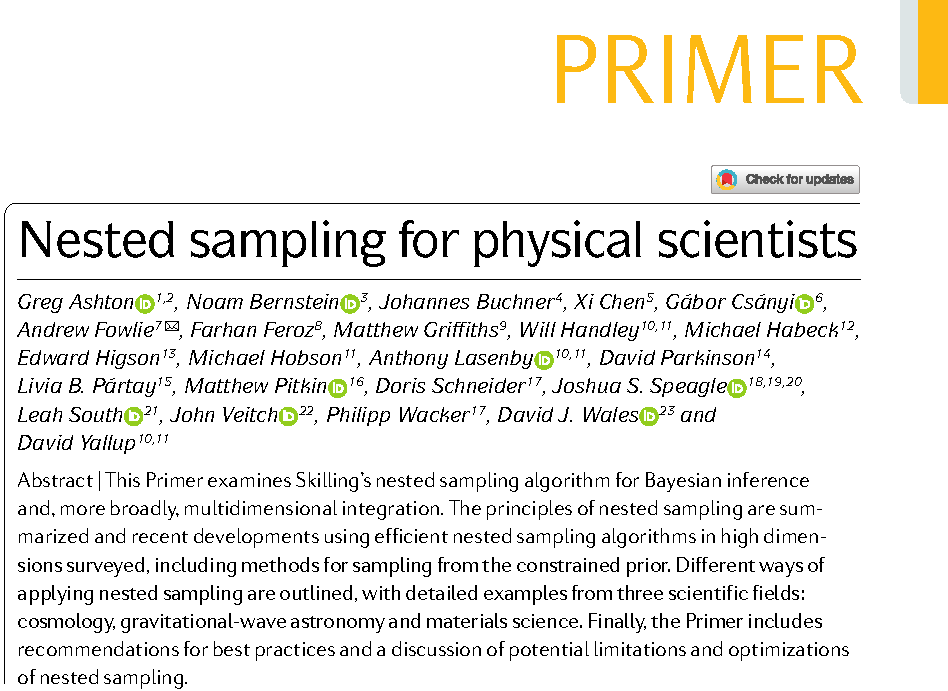
\includegraphics[width=\textwidth]{figures/nature1}
%        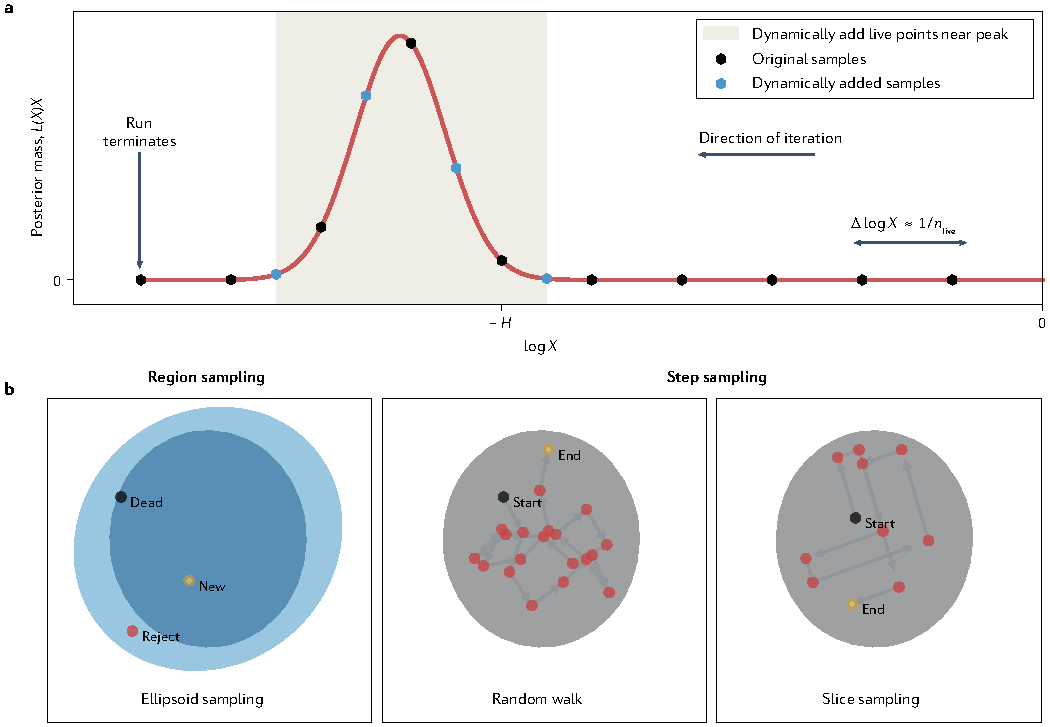
\includegraphics[width=\textwidth]{figures/nature2}
%        \column{0.2\textwidth}
%        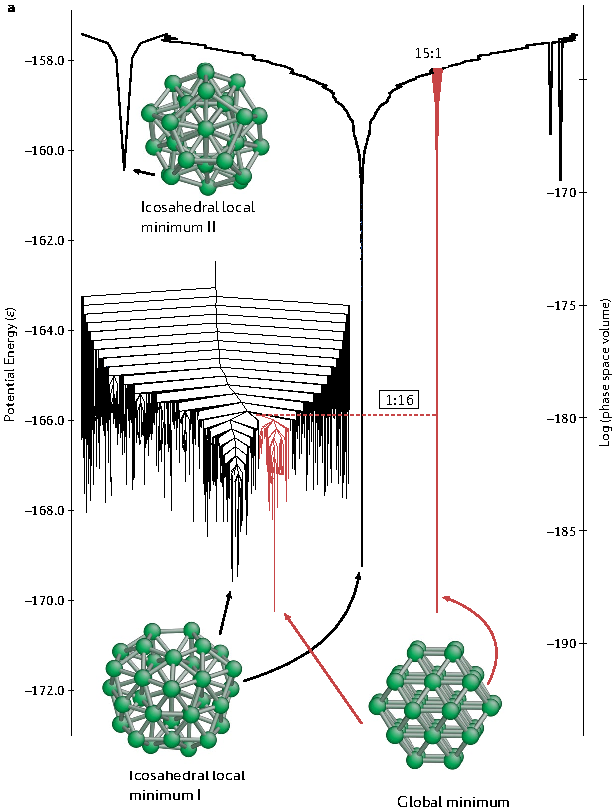
\includegraphics[width=\textwidth]{figures/nature4}
%        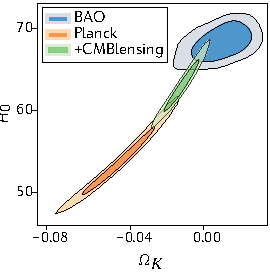
\includegraphics[width=\textwidth]{figures/nature5}
%    \end{columns}
%
%\end{frame}

\begin{frame}
    \frametitle{What is Nested Sampling?}
    \begin{itemize}
        \item Nested sampling is a radical, multi-purpose numerical tool.
        \item Given a (scalar) function $f$ with a vector of parameters $\theta$, it can be used for:
    \end{itemize}
    \vspace{-10pt}
    \begin{columns}[t]
        \column{0.3\textwidth}
        \begin{block}{Optimisation}
            \[\theta_\text{max} = \max_\theta{f(\theta)}\]
        \end{block}
        \column{0.3\textwidth}
        \begin{block}{Exploration}
            \vspace{-10pt}
            \[\text{draw/sample}\quad \theta\sim f\]
            \vspace{-15pt}
        \end{block}
        \column{0.3\textwidth}
        \begin{block}{Integration}
            \[\int f(\theta) dV \]
        \end{block}
    \end{columns}
    \begin{columns}[t]
        \column{0.33\textwidth}
        \centerline{\includegraphics[width=0.8\textwidth,page=13]{figures/himmelblau}}
        \column{0.33\textwidth}
        \centerline{\includegraphics[width=0.8\textwidth,page=15]{figures/himmelblau}}
        \column{0.33\textwidth}
        \centerline{\includegraphics[width=0.8\textwidth,page=14]{figures/himmelblau}}
    \end{columns}
\end{frame}

\begin{frame}
    \frametitle{Where is Nested Sampling?}
    \begin{columns}
        \column{0.5\textwidth}
        \begin{itemize}
            \item For many purposes, in your Neural Net you should group Nested Sampling with (MCMC) techniques such as:
                \begin{itemize}
                    \item Metropolis-Hastings (PyMC, MontePython)
                    \item Hamiltonian Monte Carlo (Stan, blackjax)
                    \item Ensemble sampling (emcee, zeus). 
                    \item Variational Inference (Pyro)
                    \item Sequential Monte Carlo 
                    \item Thermodynamic integration
                    \item Genetic algorithms
                \end{itemize}
            \item You may have heard of it branded form:
                \begin{itemize}
                    \item MultiNest
                    \item PolyChord
                    \item dynesty
                    \item ultranest
                \end{itemize}
            \end{itemize}
        \column{0.5\textwidth}
        \begin{columns}
            \column{0.5\textwidth}
        \includegraphics[width=\textwidth]{figures/emcee}
        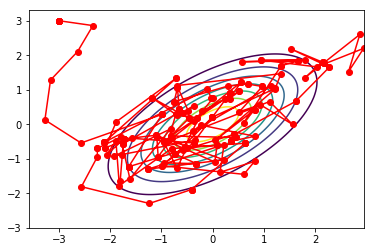
\includegraphics[width=\textwidth]{figures/metropolis-hastings}
            \column{0.5\textwidth}
        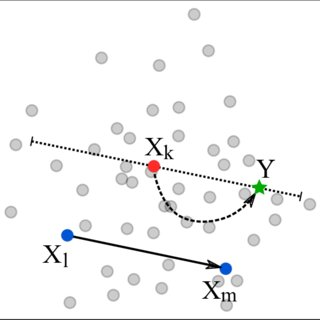
\includegraphics[width=\textwidth]{figures/zeus}
        \end{columns}
        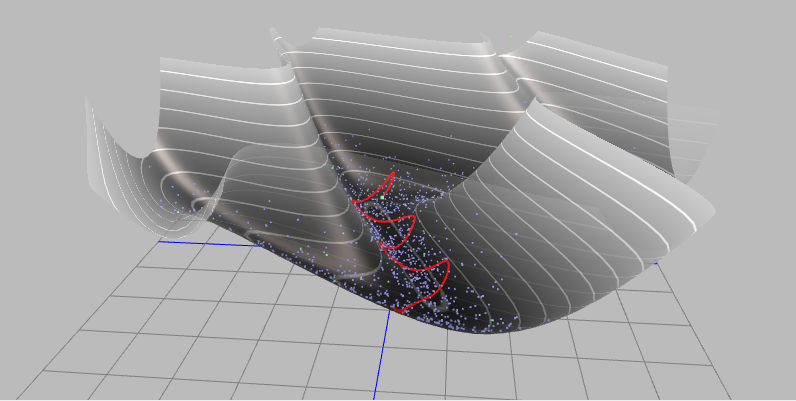
\includegraphics[width=\textwidth]{figures/hmc_explained}
    \end{columns}
\end{frame}

\begin{frame}
    \frametitle{Integration in Physics}
    \begin{itemize}
        \item Integration is a fundamental concept in physics, statistics and data science:
    \end{itemize}
    \begin{columns}
        \column{0.3\textwidth}
        \begin{block}{Partition functions}
            \vspace{-11pt}
            \[ Z(\beta) = \int e^{-\beta H(q,p)} dq dp \]
        \end{block}
        \column{0.3\textwidth}
        \begin{block}{Path integrals}
            \[ \Psi = \int e^{i S} \mathcal{D}x \]
        \end{block}
        \column{0.3\textwidth}
        \begin{block}{Bayesian marginals}
            \vspace{-11pt}
            \[ \mathcal{Z}(D) = \int \mathcal{L}(D|\theta) \pi(\theta) d\theta \]
        \end{block}
    \end{columns}
    \begin{columns}
        \column{0.6\textwidth}
        \begin{itemize}
            \item Need numerical tools if analytic solution unavailable.
            \item High-dimensional numerical integration is hard.
            \item Riemannian strategy estimates volumes geometrically:
                \[ \int f(x) d^nx \approx \sum_i f(x_i) \Delta V_i \sim \mathcal{O}(e^n) \]
            \item Curse of dimensionality $\Rightarrow$ exponential scaling.
        \end{itemize}
        \column{0.4\textwidth}
        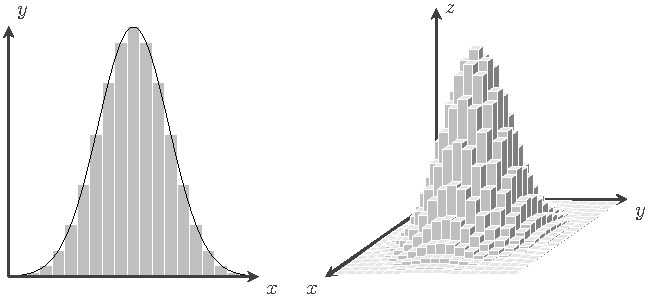
\includegraphics[width=\textwidth]{figures/integration.pdf}
    \end{columns}
\end{frame}

\begin{frame}
    \frametitle{Probabalistic volume estimation}
    \begin{columns}
        \column{0.5\textwidth}
        \begin{itemize}
            \item Key idea in NS: estimating volumes probabilistically
                \[
                    \only<-2>{
                    \frac{\C[1]{V_\mathrm{after}}}{\C[0]{V_\mathrm{before}}} 
                    \approx \frac{\C[1]{n_\mathrm{in}}}{\C[0]{n_\mathrm{out}}+\C[1]{n_\mathrm{in}}}
                }
                    \only<3>{
                    \frac{\C[1]{V_\mathrm{after}}}{\C[0]{V_\mathrm{before}}} 
                    \approx \frac{\C[1]{n_\mathrm{in}}+1}{\C[0]{n_\mathrm{out}}+\C[1]{n_\mathrm{in}}+2}
                }
                \only<4>{\hspace{-15pt}
                    \frac{\C[1]{V_\mathrm{after}}}{\C[0]{V_\mathrm{before}}} 
\sim \frac{\C[1]{n_\mathrm{in}}+1}{\C[0]{n_\mathrm{out}}+\C[1]{n_\mathrm{in}}+2} \pm \sqrt{\tfrac{(\C[1]{n_\mathrm{in}}+1)(\C[0]{n_\mathrm{out}}+1)}{(\C[0]{n_\mathrm{out}}+\C[1]{n_\mathrm{in}}+2)^2(\C[0]{n_\mathrm{out}}+\C[1]{n_\mathrm{in}}+3)}}
                }
                \]
            \item This is the \textbf{only} way to calculate volume in high dimensions $d>3$.
                \begin{itemize}
                    \item Geometry is exponentially inefficient.
                \end{itemize}
            \item This estimation process does not depend on geometry, topology or dimensionality
            \item Basis of all Monte-Carlo integration
            \item Nested Sampling uniquely uses a nested framework to couple together MC integrals in a robust, scalable manner.
        \end{itemize}
        \column{0.5\textwidth}
        \includegraphics<1>[width=\textwidth]{figures/compression_1}%
        \includegraphics<2->[width=\textwidth]{figures/compression_2}%
    \end{columns}
\end{frame}

\begin{frame}
    \begin{columns}
        \column{0.48\textwidth}
        \begin{block}{\textbf{MCMC}}
            \only<16>{
                \begin{itemize}
                    \item Single ``walker''
                    \item Explores posterior
                    \item Fast, if proposal matrix is tuned
                    \item Parameter estimation, suspiciousness calculation
                    \item Channel capacity optimised for generating posterior samples
                \end{itemize}
            }
        \end{block}
            \includegraphics<1>[width=\textwidth,page=16]{figures/himmelblau}%
            \includegraphics<2>[width=\textwidth,page=17]{figures/himmelblau}%
            \includegraphics<3>[width=\textwidth,page=18]{figures/himmelblau}%
            \includegraphics<4>[width=\textwidth,page=19]{figures/himmelblau}%
            \includegraphics<5>[width=\textwidth,page=20]{figures/himmelblau}%
            \includegraphics<6-15>[width=\textwidth,page=21]{figures/himmelblau}%
        \centerline{\includegraphics<16>[width=0.5\textwidth,page=19]{figures/himmelblau}}
        \column{0.48\textwidth}
        \begin{block}<7->{\textbf{Nested sampling}}
            \only<16>{
                \begin{itemize}
                    \item Ensemble of ``live points''
                    \item Scans from prior to peak of likelihood
                    \item Slower, no tuning required
                    \item Parameter estimation, model comparison, tension quantification
                    \item Channel capacity optimised for computing partition function
                \end{itemize}
            }
        \end{block}
            \includegraphics<7|handout:0>[width=\textwidth,page=1]{figures/himmelblau}%
            \includegraphics<8|handout:0>[width=\textwidth,page=2]{figures/himmelblau}%
            \includegraphics<9|handout:0>[width=\textwidth,page=3]{figures/himmelblau}%
            \includegraphics<10          >[width=\textwidth,page=4]{figures/himmelblau}%
            \includegraphics<11|handout:0>[width=\textwidth,page=5]{figures/himmelblau}%
            \includegraphics<12|handout:0>[width=\textwidth,page=6]{figures/himmelblau}%
            \includegraphics<13|handout:0>[width=\textwidth,page=7]{figures/himmelblau}%
            \includegraphics<14|handout:0>[width=\textwidth,page=8]{figures/himmelblau}%
            \includegraphics<15|handout:0>[width=\textwidth,page=15]{figures/himmelblau}%
        \centerline{\includegraphics<16>[width=0.5\textwidth,page=4]{figures/himmelblau}} 
    \end{columns}
\end{frame}

\begin{frame}
    \frametitle{The nested sampling meta-algorithm: live points}
    \begin{columns}
        \column{0.5\textwidth}
        \begin{itemize}
            \item Start with $n$ random samples over the space.
            \item Delete outermost sample, and replace with a new random one at higher integrand value.
            \item The ``live points'' steadily contract around the peak(s) of the function.
            \item We can use this evolution to estimate volume \emph{probabilistically}.
            \item At each iteration, the contours contract by $\sim\frac{1}{n}\only<5->{\pm \frac{1}{n}}$ of their volume.
            \item This is an exponential contraction, so
                \[  \int f(x) dV \approx \sum_i f(x_i) \Delta V_i, \quad V_i = V_0 e^{-\only<5->{(}i\only<5->{\pm\sqrt{i})}/n} \]
%            \item Nested sampling: completely different way to scan.
%            \item Ensemble sampling compresses entire space$\to$peak(s).
%            \item Sequentially update a set $S$ of $n$ samples:
%                \begin{itemize}
%                    \item[$S_0$:]  Generate $n$ samples uniformly over the space (from a measure $\pi$). 
%
%                    \item[$S_{i+1}$:] Delete the lowest likelihood sample in $S_{i}$, and replace it with a new uniform sample with higher likelihood.
%                \end{itemize}
%            \item Requires one to be able to sample uniformly within a region, subject to a {\em hard constraint}:
%                \[\{\theta\sim \pi : \mathcal{L}(\theta)>\mathcal{L}_*. \}\]
%            \item This procedure optimises (multimodally), and can calculate the \C[3]{evidence}/integral of function \& \C[0]{posterior}/sample weights.
        \end{itemize}
        \column{0.5\textwidth}
        \includegraphics<1|handout:0>[width=\textwidth,page=1]{figures/himmelblau}%
        \includegraphics<2|handout:0>[width=\textwidth,page=2]{figures/himmelblau}%
        \includegraphics<3|handout:0>[width=\textwidth,page=3]{figures/himmelblau}%
        \includegraphics<4-         >[width=\textwidth,page=4]{figures/himmelblau}%
    \end{columns}
\end{frame}

\begin{frame}
    \frametitle{The nested sampling meta-algorithm: dead points}
    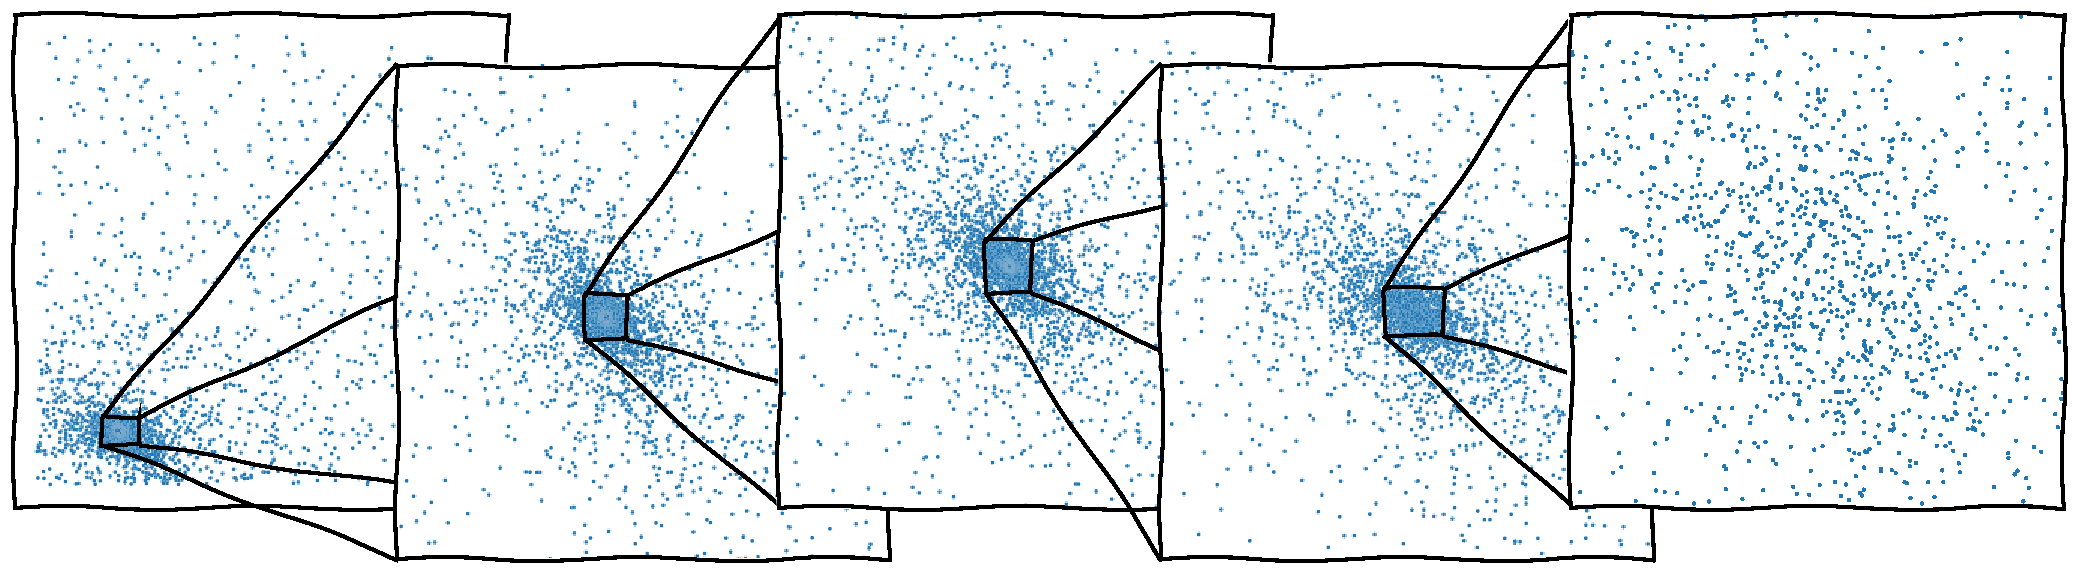
\includegraphics[width=\textwidth]{figures/dead_measure}
    \begin{columns}
        \column{0.69\textwidth}
        \begin{itemize}
            \item At the end, one is left with a set of discarded ``dead'' points.
            \item Dead points have a unique scale-invariant distribution $\propto\: \tfrac{dV}{V}$.
            \item Uniform over original region, exponentially concentrating on region of interest (until termination volume).
            \item Good for training emulators (HERA~\arxiv{2108.07282}).
        \end{itemize}
        \column{0.3\textwidth}
        \begin{block}{Applications}
        \begin{itemize}
            \item training emulators.
            \item gridding simulations
            \item beta flows
            \item ``dead measure'' 
        \end{itemize}
        \end{block}
    \end{columns}
\end{frame}


\begin{frame}
    \frametitle{The nested sampling meta-algorithm: Lebesgue integration}
    \begin{columns}
        \column{0.5\textwidth}
        \begin{itemize}
            \item Full dead-point coverage of tails enables integration.
            \item Can be weighted to form posterior samples, prior samples, or anything in between.
            \item Nested sampling estimates the \textbf{density of states} and calculates partition functions
                \[Z(\beta) = \sum_i f(x_i)^\beta \Delta V_i.\]
            \item The evolving ensemble of live points allows:
                \begin{itemize}
                    \item implementations to self-tune
                    \item exploration of multimodal functions
                    \item global and local optimisation
                \end{itemize}
            %\item Interpreted as a Bayesian algorithm, it
            %    \begin{itemize}
            %        \item Computes the Bayesian evidence (model comparison)
            %        \item Produces (weighted) posterior samples (parameter estimation)
            %    \end{itemize}
        \end{itemize}
        \column{0.5\textwidth}
        \includegraphics[width=\textwidth,page=14]{figures/himmelblau}%
        %\includegraphics<1|handout:0>[width=\textwidth,page=14]{figures/himmelblau}%
        %\includegraphics<2          >[width=\textwidth,page=15]{figures/himmelblau}%
    \end{columns}
\end{frame}

\begin{frame}
  \frametitle{Sampling from a hard likelihood constraint} 
  
  \begin{quote}
    ``It is not the purpose of this introductory paper to develop the technology of navigation within such a volume. We merely note that exploring a hard-edged likelihood-constrained domain should prove to be neither more nor less demanding than exploring a likelihood-weighted space.''
    
   {\hfill --- John Skilling}
  \end{quote}

  \begin{itemize}
      
    \item A large fraction of the work in NS to date has been in attempting to implement a hard-edged sampler in the NS meta-algorithm $\{\theta\sim \pi : \mathcal{L}(\theta)>\mathcal{L}_* \}$.
    \item \url{https://projecteuclid.org/euclid.ba/1340370944}.
    \item There has also been much work beyond this (see 'Frontiers of nested sampling' talk)
        \begin{itemize}
            \item \href{https://www.willhandley.co.uk/talks}{willhandley.co.uk/talks}
        \end{itemize}
  \end{itemize}
 
\end{frame}

\begin{frame}
    \frametitle{Implementations of Nested Sampling \arxiv{2205.15570}(NatReview)}
    %\begin{columns}
    %    \begin{column}{0.33}
    %        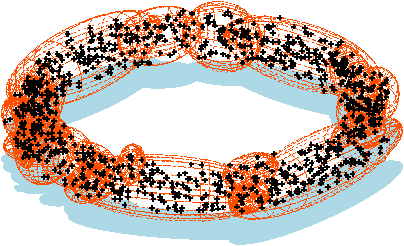
\includegraphics[width=\textwidth]{figures/multinest}
    %    \end{column} 
    %\end{columns}
    \begin{columns}[t]
        \column{0.3\textwidth}
        \texttt{MultiNest}~\arxiv{0809.3437}
        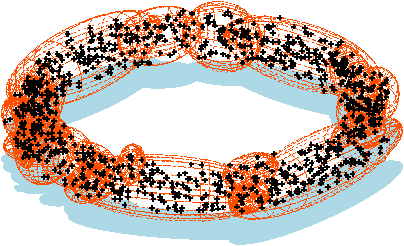
\includegraphics[width=\textwidth]{figures/multinest}
        \texttt{UltraNest}~\arxiv{2101.09604}
        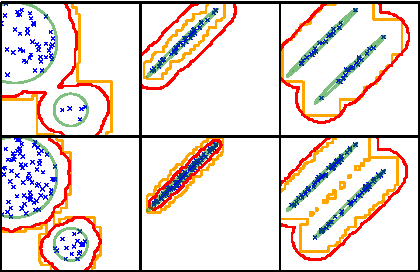
\includegraphics[width=\textwidth]{figures/radfriends}
        \texttt{nautilus}~\arxiv{2306.16923} 
        \column{0.4\textwidth}
        \texttt{PolyChord}~\arxiv{1506.00171}
        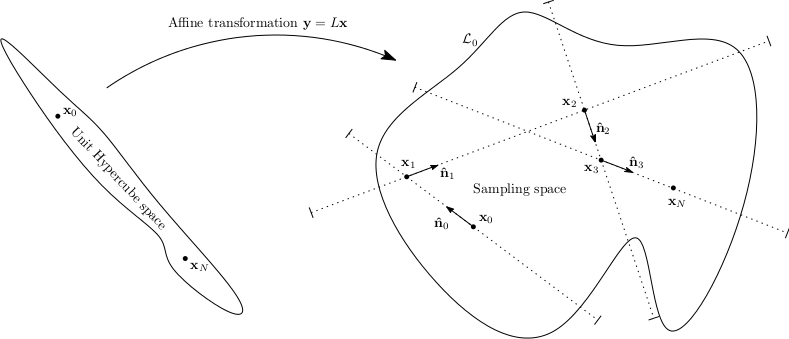
\includegraphics[width=\textwidth]{figures/polychord}
        \vfill
        \texttt{NeuralNest}~\arxiv{1903.10860}
        \begin{columns}
            \column{0.55\textwidth}
            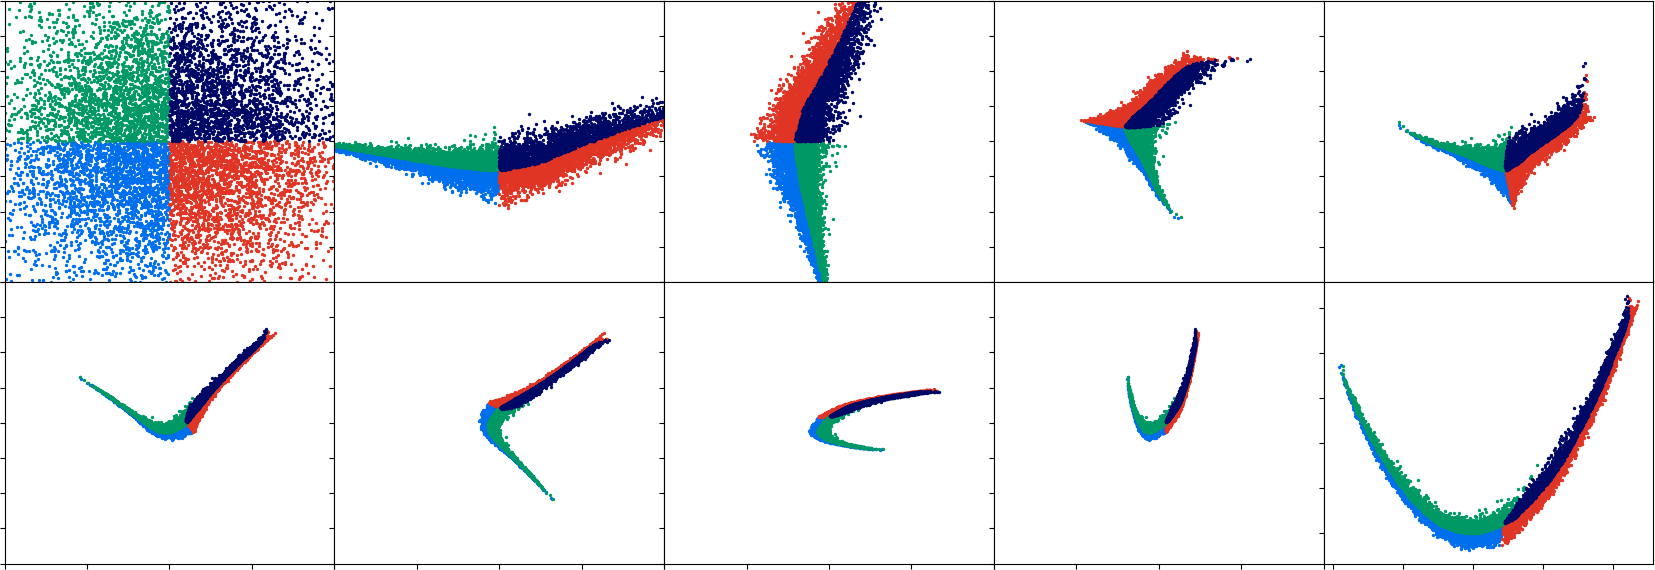
\includegraphics[width=\textwidth]{figures/rosenbrock_flow.png}
            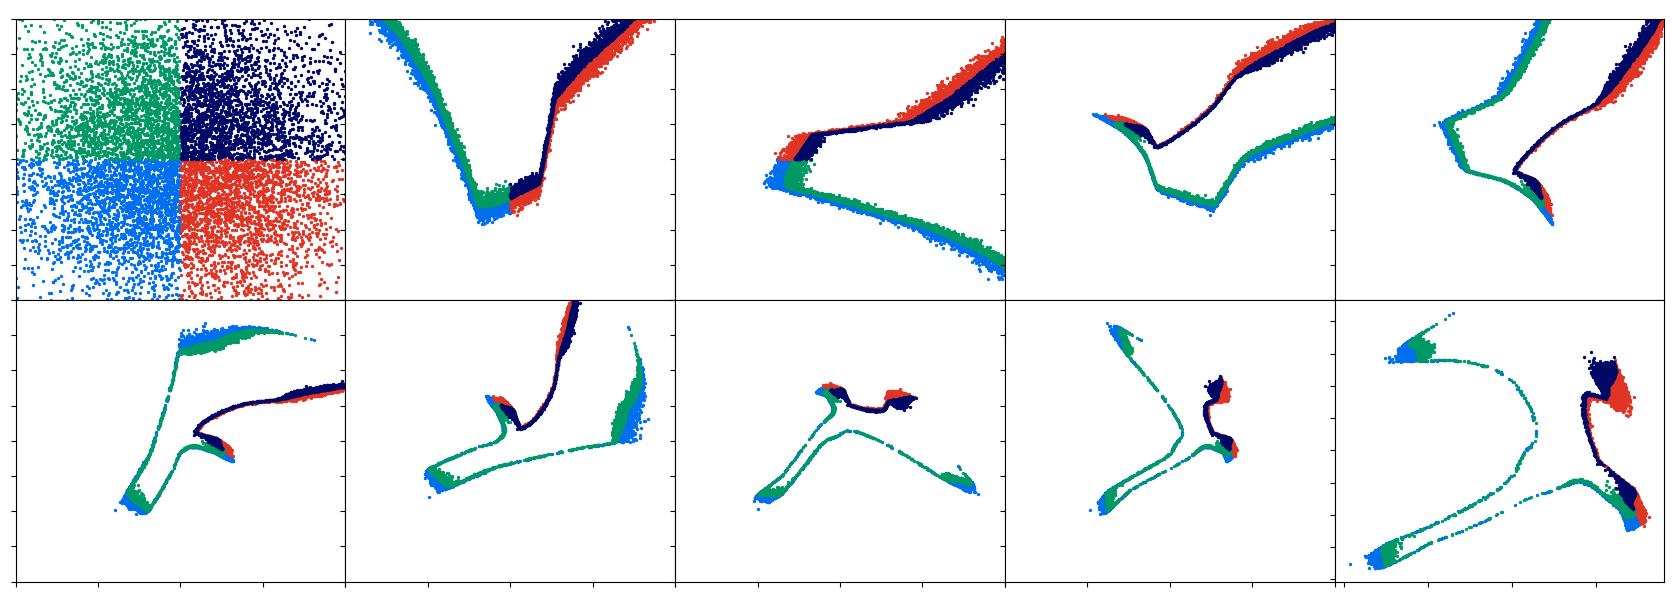
\includegraphics[width=\textwidth]{figures/himmelblau_flow.png}
            \column{0.45\textwidth}
            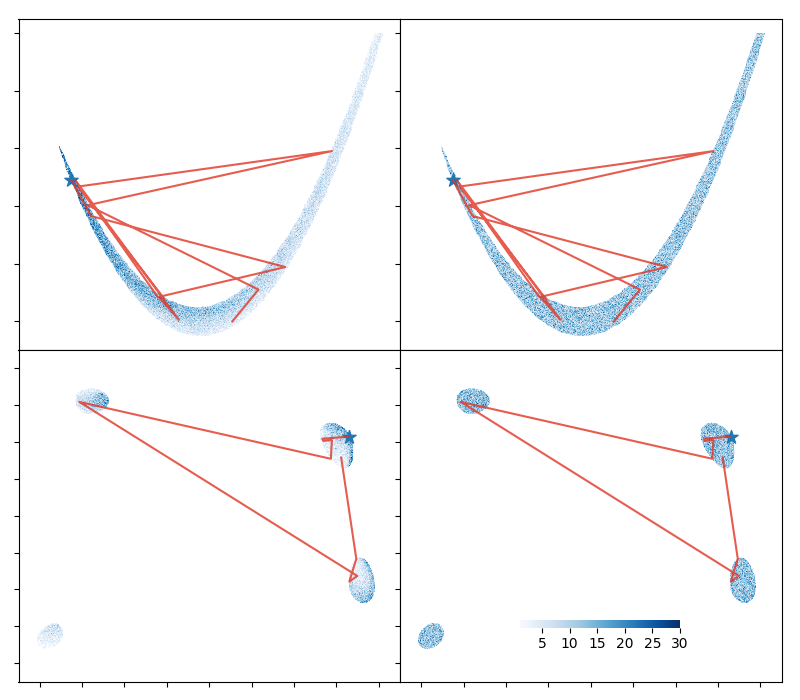
\includegraphics[width=\textwidth]{figures/chains.png}
        \end{columns}
        \texttt{nessai}~\arxiv{2102.11056} \texttt{nora}~\arxiv{2305.19267} \texttt{jaxnest}~\arxiv{2012.15286}
        \vfill
        \column{0.3\textwidth}
        \texttt{DNest}~\arxiv{1606.03757}
        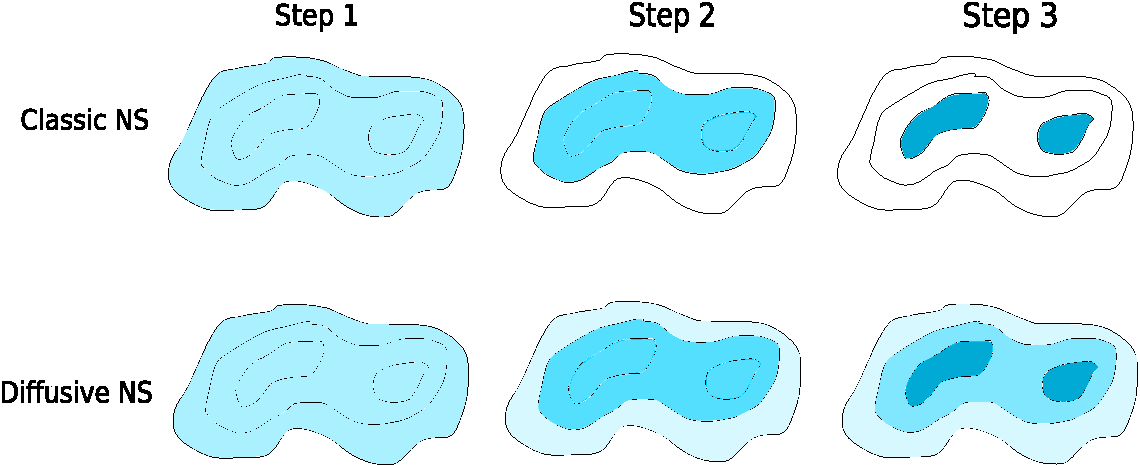
\includegraphics[width=\textwidth]{figures/dnest}
        \texttt{ProxNest}~\arxiv{2106.03646}
        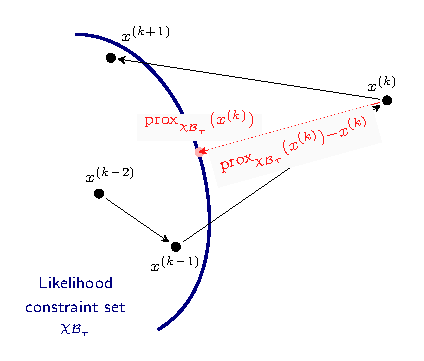
\includegraphics[width=\textwidth]{figures/proxnest_diagram}
        \texttt{dynesty}~\arxiv{1904.02180} 
        \vfill
    \end{columns}
\end{frame}

\begin{frame}
    \frametitle{Types of nested sampler}
    \begin{itemize}
        \item Broadly, most nested samplers can be split into how they create new live points.
        \item i.e. how they sample from the hard likelihood constraint $\{\theta\sim \pi : \mathcal{L}(\theta)>\mathcal{L}_* \}$.
    \end{itemize}
    \vspace{-10pt}
    \begin{columns}[t]
        \column{0.48\textwidth}
        \begin{block}{Rejection samplers}
            \begin{itemize}
                \item e.g. \texttt{MultiNest}, \texttt{UltraNest}.
\item Constructs bounding region and draws many invalid points until $\mathcal{L}(\theta)>\mathcal{L}_*$.
                \item Efficient in low dimensions, exponentially inefficient $\sim\mathcal{O}(e^{d/d_0})$ in high  $d>d_0\sim10$.
            \end{itemize}
        \end{block}
        \column{0.48\textwidth}
        \begin{block}{Chain-based samplers}
            \begin{itemize}
                \item e.g. \texttt{PolyChord}, \texttt{ProxNest}.
                \item Run Markov chain starting at a live point, generating many valid (correlated) points.
                \item Linear $\sim\mathcal{O}(d)$ penalty in decorrelating new live point from the original seed point.
            \end{itemize}
        \end{block}
    \end{columns}
    \vspace{5pt}
    \begin{itemize}
        \item Nested samplers usually come with:
            \begin{itemize}
                \item \emph{resolution} parameter $n_\mathrm{live}$ (which improve results as $\sim\mathcal{O}(n_\mathrm{live}^{-1/2})$.
                    \item set of \emph{reliability} parameters~\arxiv{2101.04525}, which don't improve results if set arbitrarily high, but introduce systematic errors if set too low.
                    \item e.g. \texttt{Multinest} efficiency \texttt{eff} or \texttt{PolyChord} chain length $n_\mathrm{repeats}$.
            \end{itemize}
    \end{itemize}
\end{frame}

\begin{frame}
    \frametitle{Applications: The three pillars of Bayesian inference}
    \begin{columns}[t]
        \column{0.33\textwidth}
        \begin{block}{Parameter estimation}
            What do the data tell us about the parameters of a model?

            \textit{e.g. the size or age of a $\Lambda$CDM universe}
            \[ \hspace{-4pt}\C[0]{P(\theta|D,M)} = \frac{\C[2]{P(D|\theta,M)} \C[1]{P(\theta|M)}}{\C[3]{P(D|M)}} \] 
            \[ \C[0]{\mathcal{P}} = \frac{\C[2]{\mathcal{L}} \times\C[1]{\pi}}{\C[3]{\mathcal{Z}}}\] 
            \[ \C[0]{\text{Posterior}} = \frac{\C[2]{\text{Likelihood}} \times\C[1]{\text{Prior}}}{\C[3]{\text{Evidence}}}\]
        \end{block}
        \column{0.3\textwidth}
        \begin{block}{Model comparison}
            How much does the data support a particular model?

            \textit{e.g. $\Lambda$CDM vs a dynamic dark energy cosmology}
            \[ \C[4]{P(M|D)} = \frac{\C[3]{P(D|M)} \C[5]{P(M)}}{\C[7]{P(D)}} \vspace{-7pt}\]
            \[ \frac{\C[3]{\mathcal{Z}_\mathcal{M}} \C[5]{\Pi_\mathcal{M}}}{\C[7]{\sum_m Z_m \Pi_m}} \]
            \[ \C[4]{\text{Posterior}} = \frac{\C[3]{\text{Evidence}} \times\C[5]{\text{Prior}}}{\C[7]{\text{Normalisation}}}\]
        \end{block}
        \column{0.33\textwidth}
        \begin{block}{Tension quantification}
            Do different datasets make consistent predictions from the same model? 
            \textit{e.g. CMB vs Type IA supernovae data}
            \[ \mathcal{R} = \frac{\C[3]{\mathcal{Z}}_{AB}}{\C[3]{\mathcal{Z}}_A\C[3]{\mathcal{Z}}_\mathcal{B}}\] 
            \[
                \begin{aligned} \log\mathcal{S} = \av[{\C[0]{\mathcal{P}}_{AB}}]{\C[2]{\log\mathcal{L}}_{AB}}&\\
                    -\av[{\C[0]{\mathcal{P}}_{A}}]{\C[2]{\log\mathcal{L}}_{A}}&\\
                    -\av[{\C[0]{\mathcal{P}}_{B}}]{\C[2]{\log\mathcal{L}}_{B}}&
                \end{aligned}
            \]
        \end{block}
    \end{columns}
\end{frame}

\begin{frame}
    \frametitle{Applications of nested sampling}
    \framesubtitle{Cosmology}
    \student{adam_ormondroyd}{Adam Ormondroyd}{PhD}
    \begin{columns}
        \column{0.55\textwidth}
        \begin{itemize}
            \item Battle-tested in Bayesian cosmology on
                \begin{itemize}
                    \item Parameter estimation: multimodal alternative to MCMC samplers.
                    \item Model comparison: using integration to compute the Bayesian evidence
                    \item Tension quantification: using deep tail sampling and suspiciousness computations.
                \end{itemize}
            \item Plays a critical role in major cosmology pipelines: Planck, DES, KiDS, BAO, SNe.
            \item The default $\Lambda$CDM cosmology is well-tuned to have Gaussian-like posteriors for CMB data. 
            \item Less true for alternative cosmologies/models and orthogonal datasets, so nested sampling crucial.
        \end{itemize}
        \column{0.45\textwidth}
        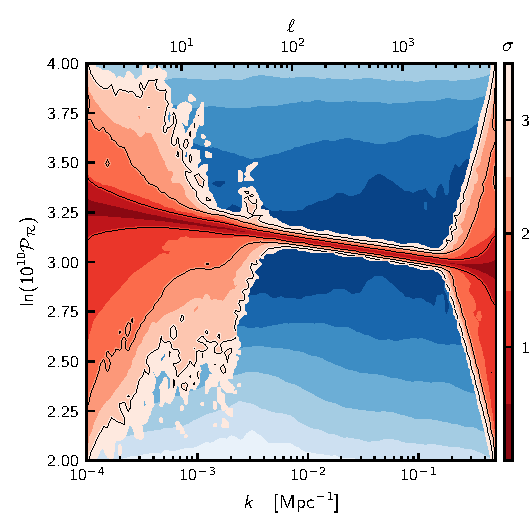
\includegraphics[width=0.49\textwidth]{figures/pps_both}
        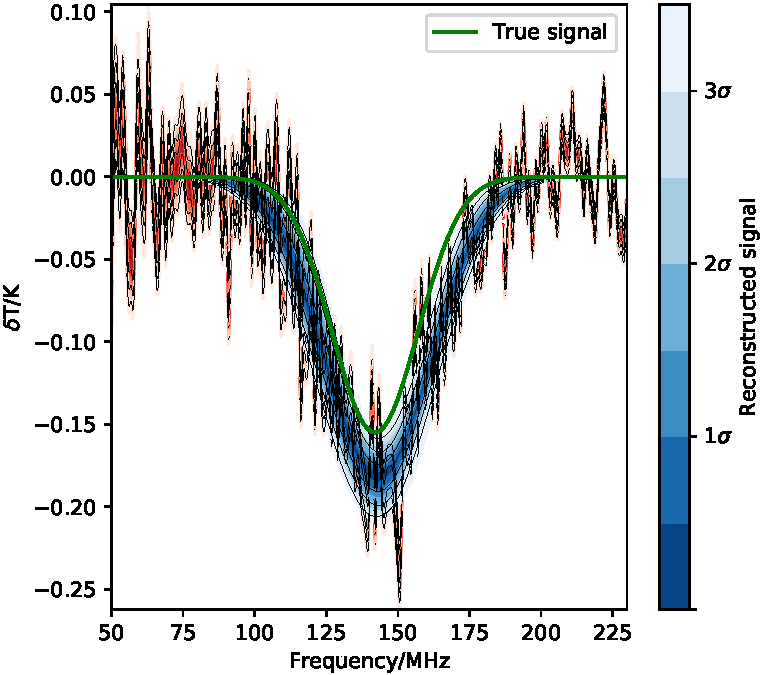
\includegraphics[width=0.49\textwidth]{figures/reach_fit-cropped.pdf}
        %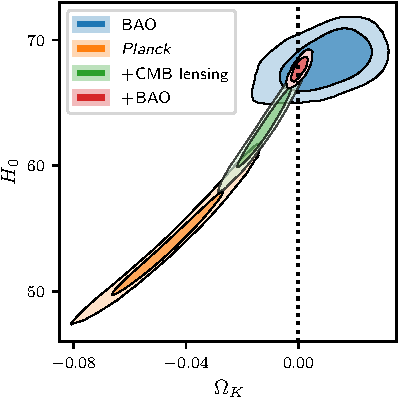
\includegraphics[width=0.49\textwidth]{figures/curvature_3}
        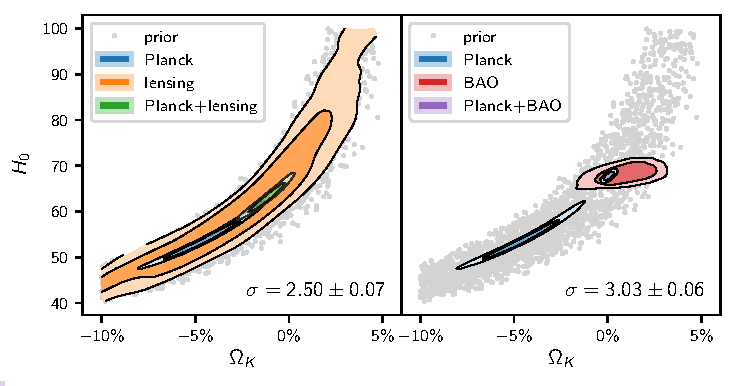
\includegraphics[width=\textwidth]{figures/omegak_H0_2.pdf}
    \end{columns}
\end{frame}

\begin{frame}
    \frametitle{Applications of nested sampling}
    \framesubtitle{Astrophysics}
\student{metha_prathaban}{Metha Prathaban}{PhD}
    \begin{columns}
        \column{0.6\textwidth}
        \begin{itemize}
            \item In exoplanets~\arxiv{1806.00518}
                \begin{itemize}
                    \item Parameter estimation: determining properties of planets.
                    \item Model comparison: how many planets? Stellar modelling~\arxiv{2007.07278}.
                    \item exoplanet problems regularly have posterior phase transitions \arxiv{2102.03387}
                \end{itemize}
            \item In gravitational waves
                \begin{itemize}
                    \item Parameter estimation: Binary merger properties
                    \item Model comparison: Modified theories of gravity, selecting phenomenological parameterisations~\arxiv{1803.10210}
                    \item Likelihood reweighting: fast slow properties
                \end{itemize}
        \end{itemize}
        \column{0.4\textwidth}
        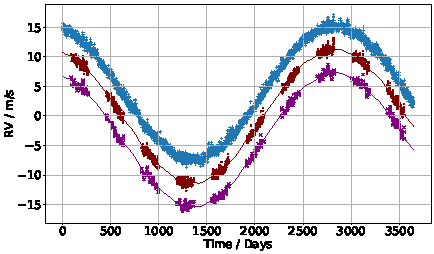
\includegraphics[width=\textwidth]{figures/rv_full.pdf}
        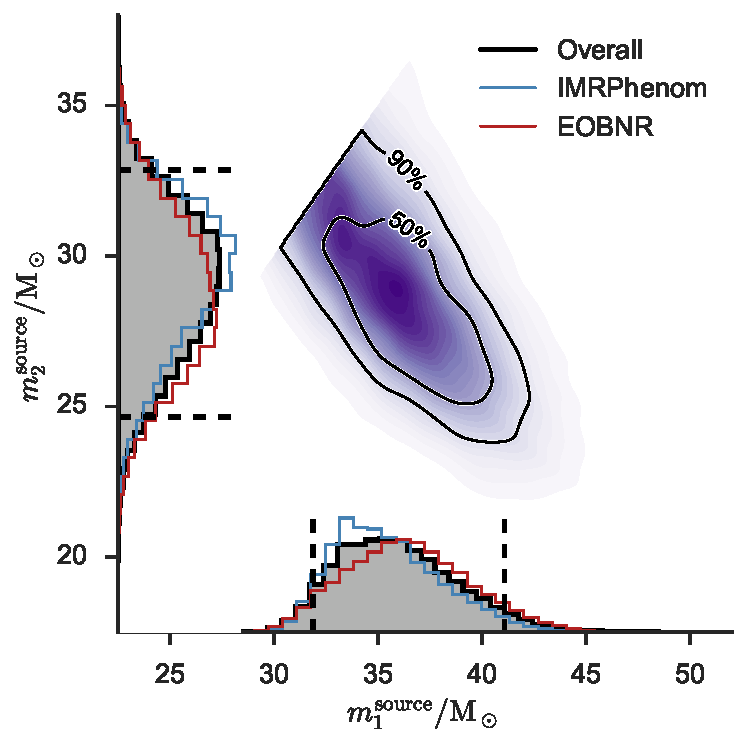
\includegraphics[width=0.49\textwidth]{figures/ligo_m1_m2.pdf}
        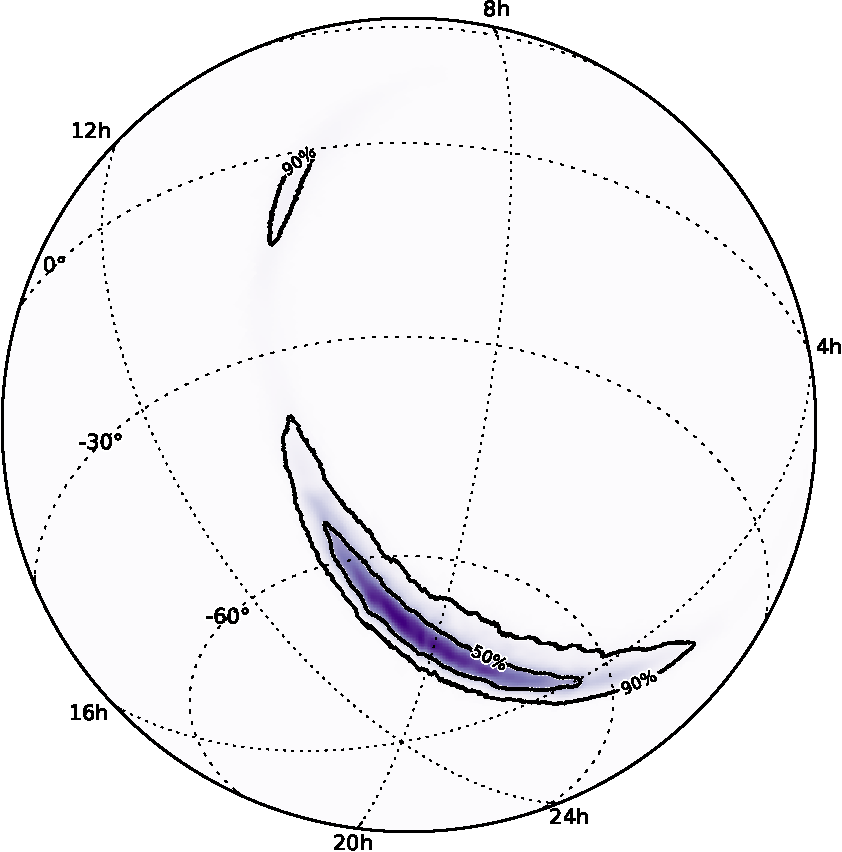
\includegraphics[width=0.49\textwidth]{figures/ligo_lambert-skymap.pdf}
    \end{columns}
\end{frame}

\begin{frame}
    \frametitle{Applications of nested sampling}
    \framesubtitle{Particle physics}
    \student{david_yallup}{David Yallup}{PDRA}
    \begin{columns}
        \column{0.56\textwidth}
        \begin{columns}
            \column{0.67\textwidth}
            \begin{itemize}
                \item Nested sampling for cross section computation/event generation
            \end{itemize}
            \column{0.3\textwidth}
            \[\sigma = \int_\Omega d\Phi |\mathcal{M}|^2.\]
        \end{columns}
        \begin{itemize}
            \item Nested sampling can explore the phase space $\Omega$ and compute integral blind with comparable efficiency to HAAG/RAMBO~\arxiv{2205.02030}.
            \item Bayesian sparse reconstruction~\arxiv{1809.04598} applied to bump hunting allows evidence-based detection of signals in phenomenological backgrounds~\arxiv{2211.10391}.
            \item Fine tuning quantification
            \item Fast estimation of small $p$-values \arxiv{2106.02056}(PRL), just make switch:\\ $X\leftrightarrow p$, $\mathcal{L}\leftrightarrow\lambda$, $\theta \leftrightarrow x$.

        \end{itemize}
        \column{0.17\textwidth}
        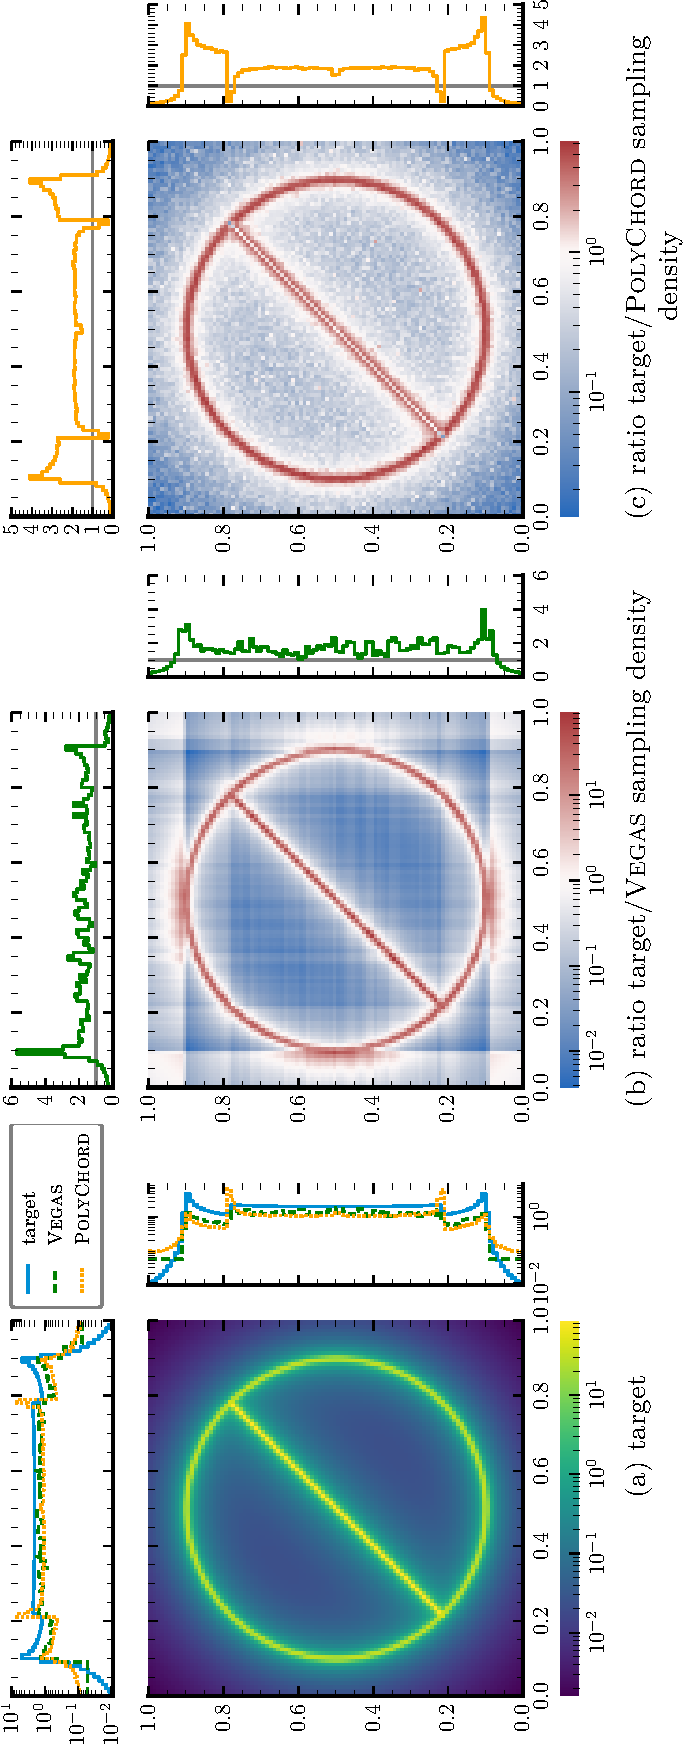
\includegraphics[width=\textwidth]{figures/phase_space_1-pdfjam-crop.pdf}
        \column{0.27\textwidth}
        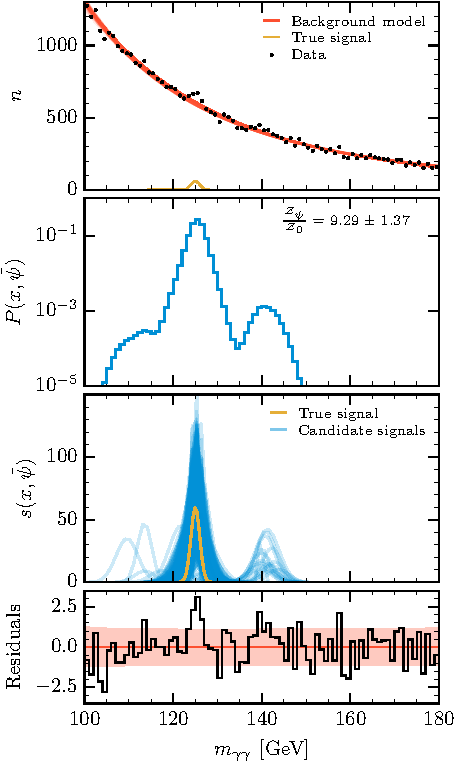
\includegraphics[width=\textwidth]{figures/psi_predict-crop.pdf}
    \end{columns}
\end{frame}


\begin{frame}
    \frametitle{Applications of nested sampling}
    \framesubtitle{Lattice field theory}
\student{david_yallup}{David Yallup}{PDRA}
    \begin{columns}
        \column{0.5\textwidth}
        \begin{itemize}
            \item Consider standard field theory Lagrangian:
                \[ Z(\beta) = \int D\phi e^{-\beta S(\phi)}, \quad S(\phi) = \int dx^\mu \mathcal{L}(\phi) \]
            \item Discretize onto spacetime grid.
            \item Compute partition function
            \item NS unique traits:
                \begin{itemize}
                    \item Get full partition function for free
                    \item allows for critical tuning
                    \item avoids critical slowing down
                \end{itemize}
            \item Applications in lattice gravity, QCD, condensed matter physics
            \item Publication imminent (next week)
        \end{itemize}
        \column{0.5\textwidth}
        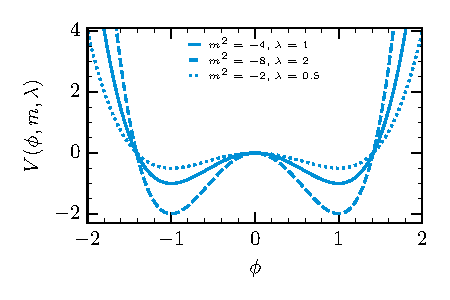
\includegraphics[width=0.49\textwidth]{figures/potential_shape}
        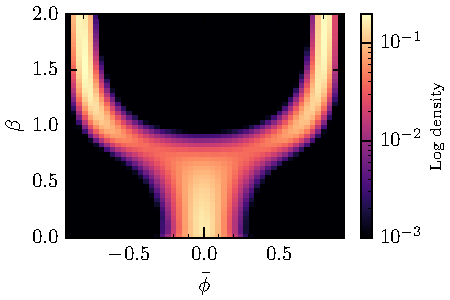
\includegraphics[width=0.49\textwidth]{figures/2d_phase}
        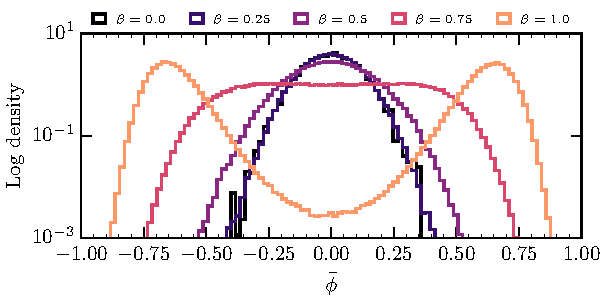
\includegraphics[width=\textwidth]{figures/lattice_field_theory.pdf}
    \end{columns}
\end{frame}
\begin{frame}
    \frametitle{Applications of nested sampling}
    \framesubtitle{Machine learning}
\student{kamran_javid}{Kamran Javid}{PDRA}
    \begin{columns}
        \column{0.62\textwidth}
        \begin{itemize}
            \item Machine learning requires:
                \begin{itemize}
                    \item Training to find weights
                    \item Choice of architecture/topology/hyperparameters
                \end{itemize}
            \item Bayesian NNs treat training as a model fitting problem
            \item Compute posterior of weights (parameter estimation), rather than optimisation (gradient descent)
            \item Use evidence to determine best architecture (model comparison), correlates with out-of-sample performance! 
            \item Solving the full ``shallow learning'' problem without compromise \arxiv{2004.12211}\arxiv{2211.10391}. 
                \begin{itemize}
                    \item Promising work ongoing to extend this to transfer learning and deep nets.
                \end{itemize}
            \item More generally, dead points are optimally spaced  for training traditional ML approaches e.g. \arxiv{2309.05697}
        \end{itemize}
        \column{0.38\textwidth}
        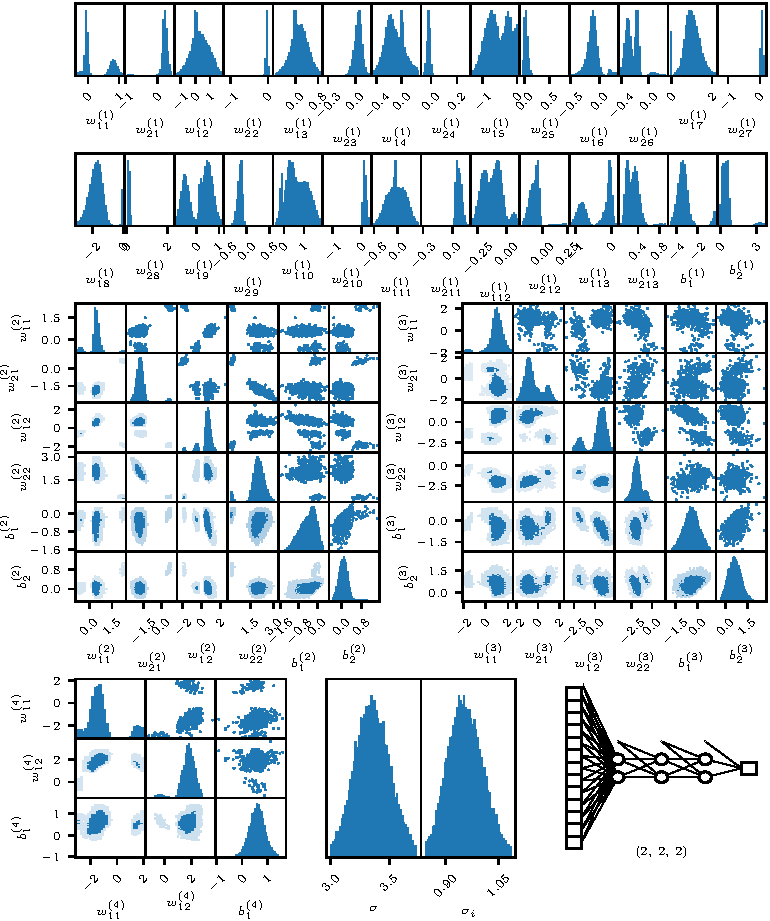
\includegraphics[width=\textwidth]{figures/nn_posterior-cropped.pdf}
    \end{columns}
\end{frame}

%\begin{frame}
%    \frametitle{Applications of nested sampling}
%    \framesubtitle{Statistics: fast estimation of small $p$-values~\arxiv{2106.02056}(PRL)}
%    \begin{columns}
%        \column{0.57\textwidth}
%        \begin{itemize}
%            \item Nested sampling for frequentist computation!?
%            \item $p$-value: $P(\lambda>\lambda^*|H_0)$ -- probability that test statistic $\lambda$ is at least as great as observed $\lambda^*$.
%            \item Computation of a tail probability from sampling distribution of $\lambda$ under $H_0$.
%            \item For gold-standard $5\sigma$, this is very expensive to simulate directly ($\sim10^9$ by definition).
%            \item Need insight/approximation to make efficient.
%            \item Nested sampling is tailor-made for this, just make switch: $X\leftrightarrow p$, $\mathcal{L}\leftrightarrow\lambda$, $\theta \leftrightarrow x$.
%            \item The only real conceptual shift is switching the integrator from parameter- to data-space.
%        \end{itemize}
%        \column{0.43\textwidth}
%        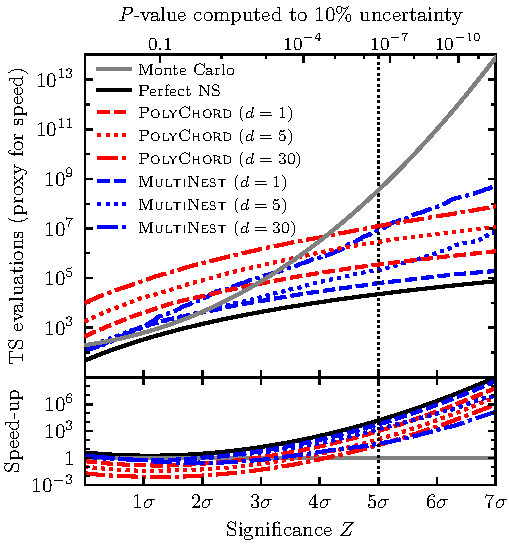
\includegraphics[width=\textwidth]{figures/pvalue.pdf}
%    \end{columns}
%\end{frame}

\begin{frame}
    \frametitle{Applications of nested sampling}
    \framesubtitle{And beyond\ldots}
    \only<1-4>{
        \student{watkinson-headshot}{Catherine Watkinson}{Senior Data Scientist}
    }
    \only<5->{
        \student{mcaloone-headshot}{Thomas Mcaloone}{PhD $\to$ Data Scientist}
    }
    \begin{columns}
        \column{0.6\textwidth}
        \begin{itemize}
            \item Techniques have been spun-out (PolyChord Ltd) to:
            \item Protein folding
                \begin{itemize}
                    \item Navigating free energy surface.
                    \item Computing misfolds.
                    \item Thermal motion.
                \end{itemize}
            \item Nuclear fusion reactor optimisation
                \begin{itemize}
                    \item multi-objective.
                    \item uncertainty propagation.
                \end{itemize}
            \item Telecoms \& DSTL research (MIDAS)
                \begin{itemize}
                    \item Optimising placement of transmitters/sensors.
                    \item Maximum information data acquisition strategies.
                \end{itemize}
        \end{itemize}
            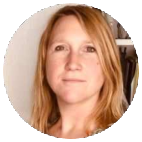
\includegraphics[width=0.08\textwidth]{figures/headshots/catherine-watkinson.pdf}%
            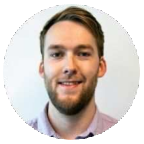
\includegraphics[width=0.08\textwidth]{figures/headshots/thomas-macaloone.pdf}%
            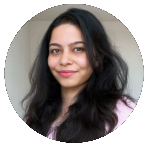
\includegraphics[width=0.08\textwidth]{figures/headshots/parul-janagal.pdf}%
            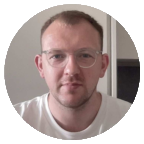
\includegraphics[width=0.08\textwidth]{figures/headshots/angus-peters.pdf}%
            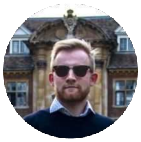
\includegraphics[width=0.08\textwidth]{figures/headshots/tamas-stenzel.pdf}%
            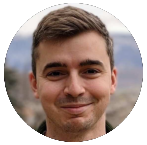
\includegraphics[width=0.08\textwidth]{figures/headshots/david-yallup.pdf}%
            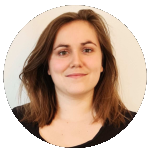
\includegraphics[width=0.08\textwidth]{figures/headshots/rebecca-handley.pdf}%
            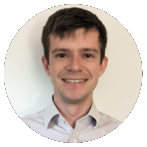
\includegraphics[width=0.08\textwidth]{figures/headshots/adam-ormondroyd.pdf}%
            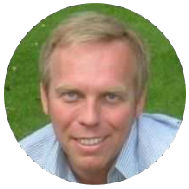
\includegraphics[width=0.08\textwidth]{figures/headshots/mike-hobson.pdf}%
            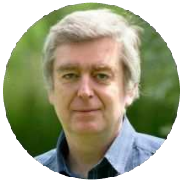
\includegraphics[width=0.08\textwidth]{figures/headshots/anthony-lasenby.pdf}%
            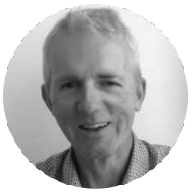
\includegraphics[width=0.08\textwidth]{figures/headshots/mike-handley.pdf}%
            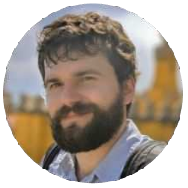
\includegraphics[width=0.08\textwidth]{figures/headshots/will-handley.pdf}%
        \column{0.4\textwidth}
        \includegraphics<1|handout:0>[width=\textwidth]{figures/protein_1.png}%
        \includegraphics<2          >[width=\textwidth]{figures/protein_2.png}%
        \includegraphics<3|handout:0>[width=\textwidth]{figures/protein_3.png}%
        \includegraphics<4|handout:0>[width=\textwidth]{figures/lcoe.png}%
        %\includegraphics<5|handout:0>[width=\textwidth]{figures/tdoa-cropped-1-crop.pdf}%
        %\includegraphics<6|handout:0>[width=\textwidth]{figures/tdoa-cropped-2-crop.pdf}%
        %\includegraphics<7|handout:0>[width=\textwidth]{figures/tdoa-cropped-3-crop.pdf}%
        \includegraphics<5|handout:0>[width=\textwidth]{figures/DKL_contour-cropped-crop.pdf}%
        \includegraphics<6|handout:0>[width=\textwidth]{figures/mean_DKL_optimise-3-crop.pdf}%
        \includegraphics<7|handout:0>[width=\textwidth]{figures/mean_DKL_optimise-4-crop.pdf}%
        \includegraphics<8|handout:0>[width=\textwidth]{figures/mean_DKL_optimise-5-crop.pdf}%
    \end{columns}
\end{frame}

\begin{frame}
    \frametitle{REACH: Global 21cm cosmology {\small \arxiv{2210.07409}(NatAstro)}}
    \student{ian_roque}{Ian Roque}{PhD}
    \vspace{10pt}
    \begin{columns}
        \column{0.65\textwidth}
        \vspace{-10pt}
        \begin{itemize}
            \item Imaging the universal dark ages using CMB backlight.
            \item $21\text{cm}$ hyperfine line emission from neutral hydrogen.
            \item Global experiments measure monopole across frequency.
            \item Challenge: science hidden in foregrounds $\sim 10^4\times$signal.
            \item Lead data analysis team (REACH first light in January)
            \item Nested sampling woven in from the ground up (calibrator, beam modelling, signal fitting, likelihood selection).
            \item All treated as parameterised model comparison problems.
        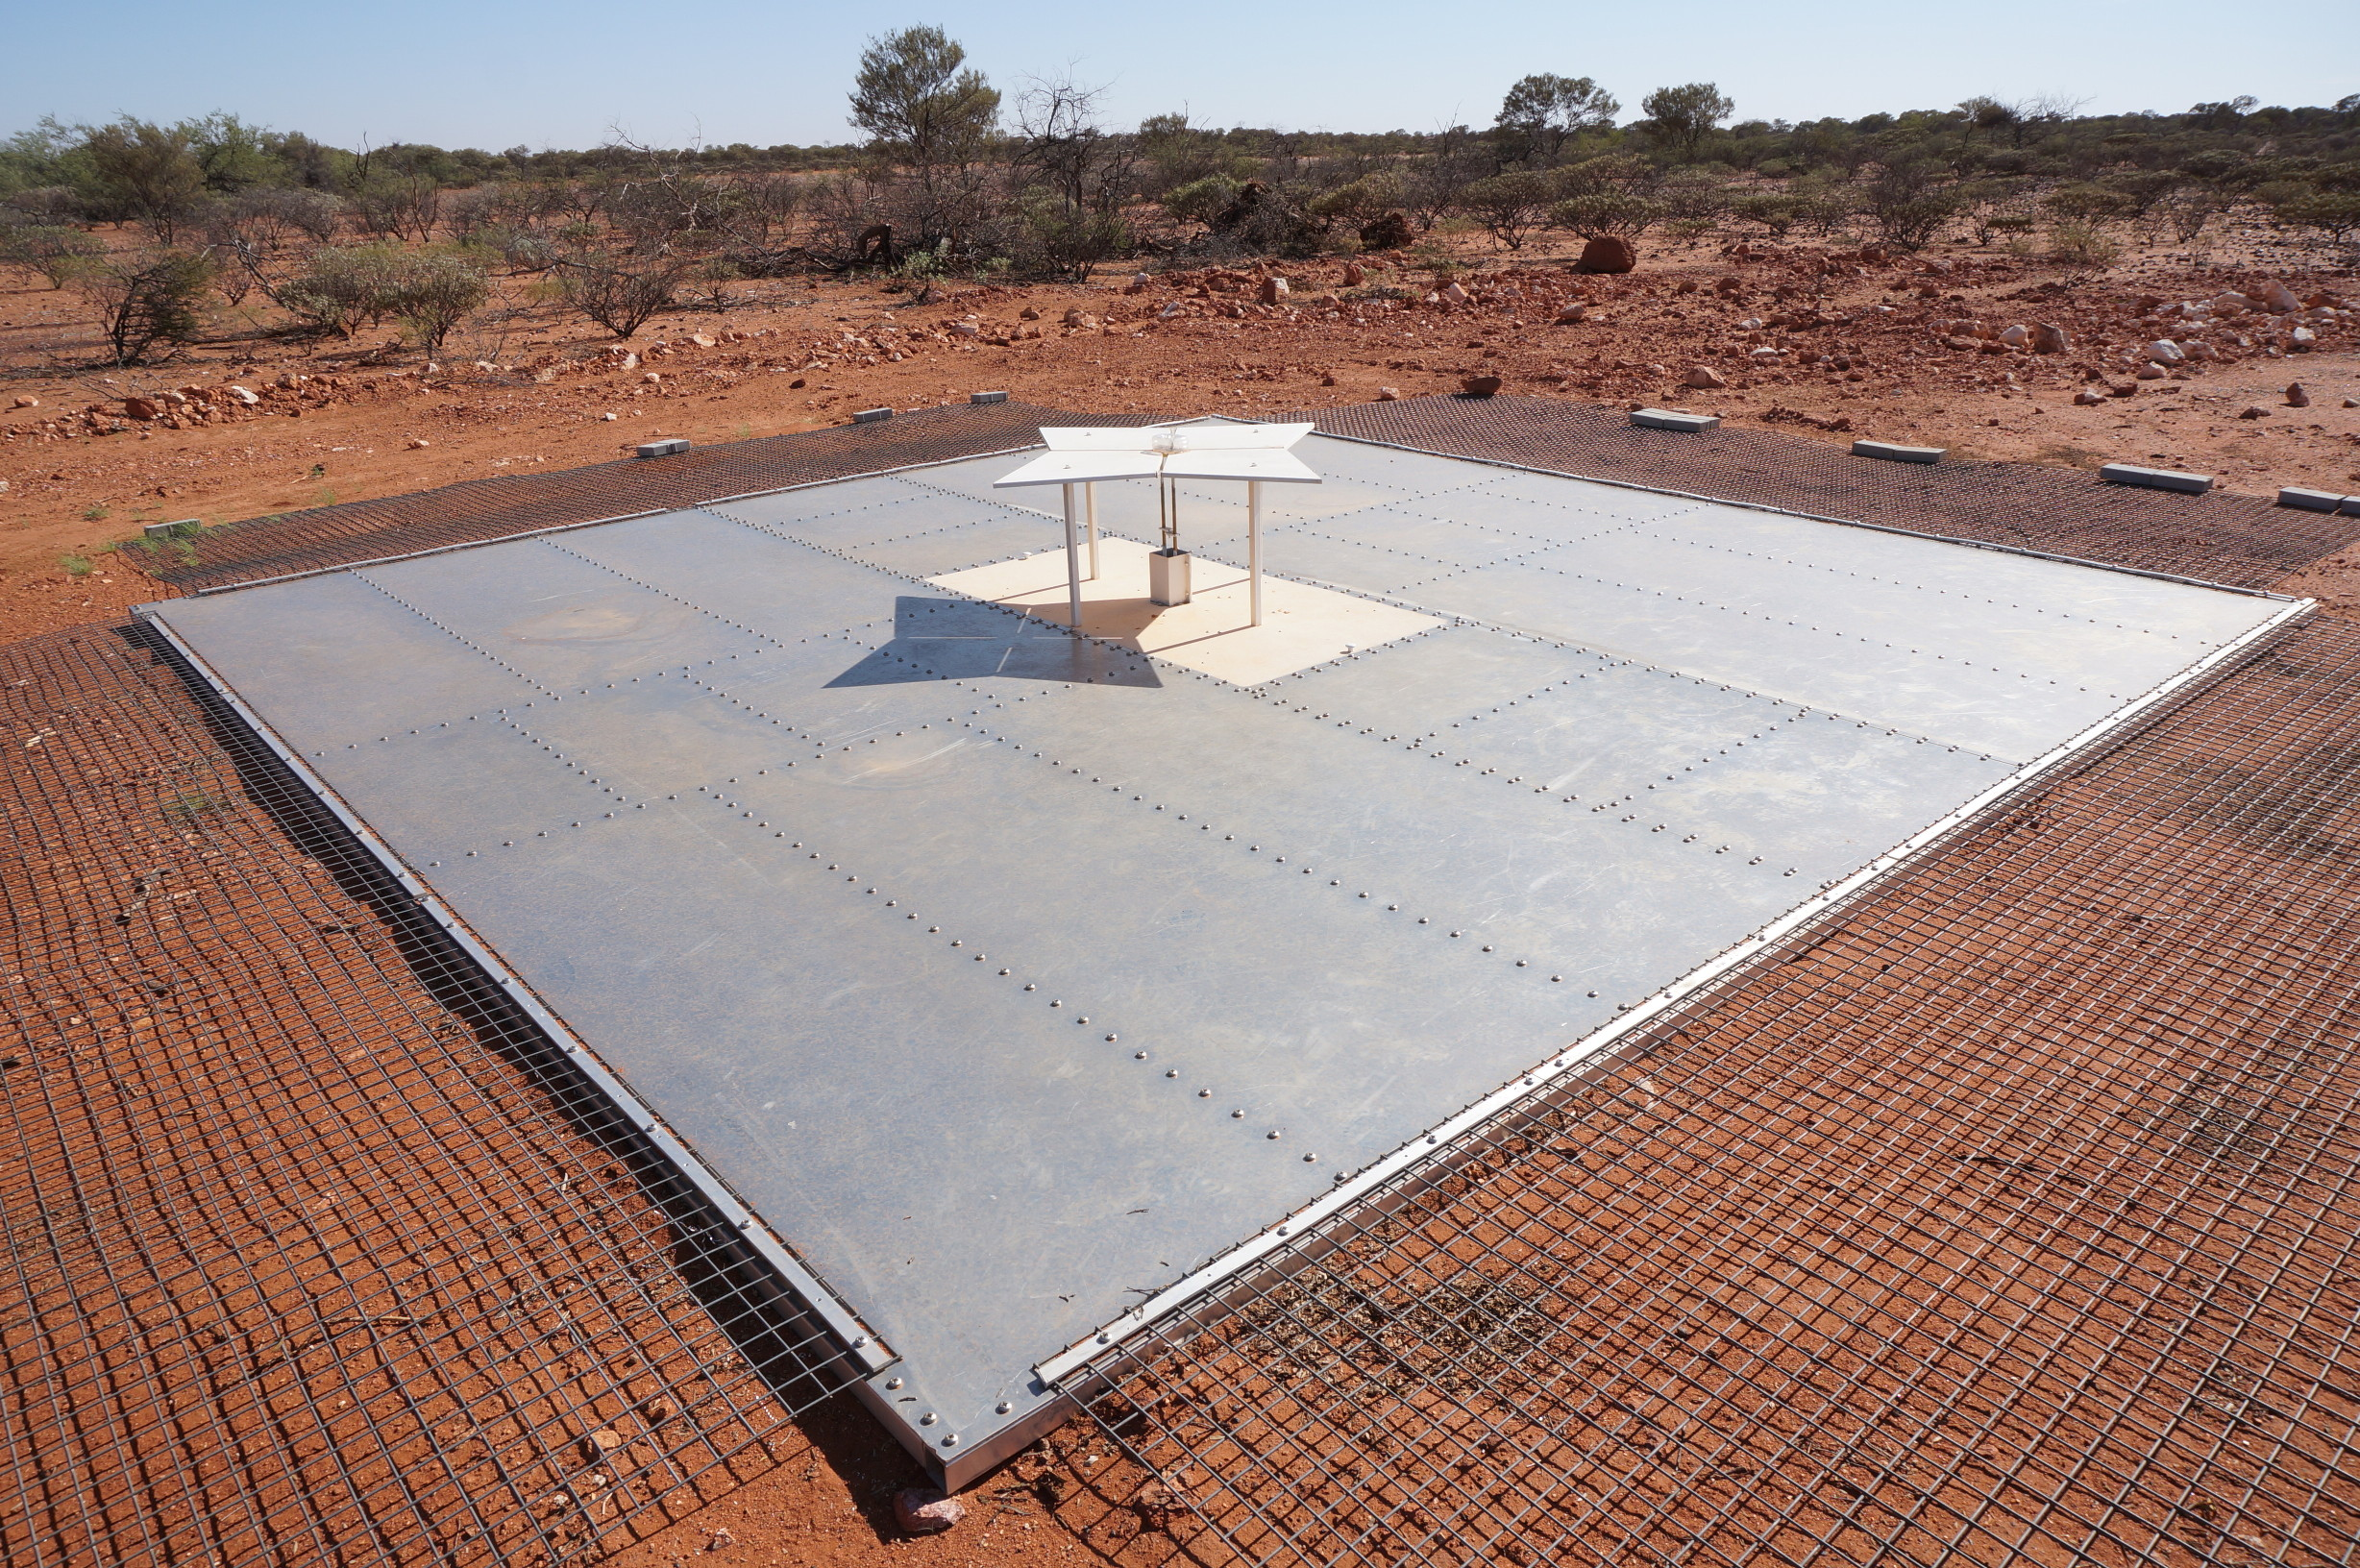
\includegraphics[height=0.3\textwidth]{figures/EDGES_antenna}
        \includegraphics[height=0.3\textwidth]{figures/SARAS}
        \includegraphics[height=0.3\textwidth]{figures/REACH_2.jpg}
        \end{itemize}
        \column{0.35\textwidth}
        \includegraphics[width=\textwidth]{figures/21cm_1.png}
        \includegraphics[width=\textwidth]{figures/21cm.png}
    \end{columns}
\end{frame}

\begin{frame}
    \frametitle{GAMBIT: combining particle physics \& cosmological data}
    \begin{columns}
        \column{0.52\textwidth}
        \begin{itemize}
            \item Multinational team of particle physicists, cosmologists and statisticians.
            \item Combine cosmological data, particle colliders, direct detection, \& neutrino detectors in a statistically principled manner~\arxiv{2205.13549}.
            \item Lead Cosmo/Dark Matter working group~\arxiv{2009.03286}.
            \item Nested sampling used for global fitting, and fine-tuning quantification~\arxiv{2101.00428}
        \end{itemize}
        \begin{center}
            \includegraphics[width=0.5\textwidth]{figures/gambit_logo.png}
        \end{center}
        \column{0.48\textwidth}
        \vspace{-40pt}
        \includegraphics[width=\textwidth]{figures/ALP_2.pdf}
    \end{columns}
\end{frame}
\begin{frame}
    \frametitle{Likelihood-free inference (aka SBI)}
\student{kilian_scheutwinkel}{Kilian Scheutwinkel}{PhD}

    \vspace{10pt}
    \begin{columns}
        \column{0.5\textwidth}
        \vspace{-10pt}
        \begin{itemize}
            \item How do you do inference if you don't know the likelihood $P(D|\theta)$?
                \begin{itemize}
                    \item e.g.\ if you can simulate a disease outbreak, how can you infer a posterior on $R_0$, or select the most predictive model?
                \end{itemize}
            \item If you can forward simulate/model $\theta\to D$, then you have an implicit likelihood.
            \item LFI aims to (machine-)\emph{learn} the likelihood from forward simulations $\{(\theta,D)\}$.
            \item Nested sampling has much to offer
                \begin{itemize}
                    \item truncation strategies (\texttt{PolySwyft})
                    \item evidence driven compression
                    \item marginalised machine learning
                \end{itemize}
            \item In my view, LFI represents the future of inference -- in twenty years time this will be as well-used as MCMC techniques are today.
        \end{itemize}
        \column{0.5\textwidth}
        \includegraphics[width=\textwidth]{figures/noisy.pdf}
        \includegraphics[width=\textwidth]{figures/three_ways_II.pdf}
    \end{columns}
\end{frame}

\begin{frame}
    \frametitle{unimpeded: PLA for the next generation}
\student{harry_bevins}{Harry Bevins}{PhD$\to$JRF}
    \begin{columns}
        \column{0.5\textwidth}
        \begin{itemize}
            \item DiRAC 2020 RAC allocation of 30MCPUh
            \item Main goal: Planck Legacy Archive equivalent
            \item Parameter estimation $\to$ Model comparison
            \item MCMC $\to$ Nested sampling
            \item Planck $\to$ $\{\text{Planck}, \text{DESY1}, \text{BAO}, \ldots \}$
            \item Pairwise combinations
            \item Suite of tools for processing these 
                \begin{itemize}
                    \item \texttt{anesthetic} $2.0$
                    \item \texttt{unimpeded} $1.0$
                    \item \texttt{zenodo} archive
                    \item \texttt{margarine}
                \end{itemize}
            \item MCMC chains also available.
            \item Library of bijectors emulators for fast re-use
        \end{itemize}
        \column{0.5\textwidth}
        \includegraphics[width=\textwidth]{logos/dirac}
        \includegraphics[width=0.5\textwidth,page=21]{figures/himmelblau}%
        \includegraphics[width=0.5\textwidth,page=15]{figures/himmelblau}
    \end{columns}
\end{frame}

\begin{frame}
    \frametitle{CosmoTension}
    \framesubtitle{Resolving cosmological tensions with diverse data, novel theories and Bayesian machine learning}
\student{will_barker}{Will Barker}{PhD$\to$JRF}
    \begin{columns}
        \column{0.6\textwidth}
        \begin{itemize}
            \item ERC grant $\Rightarrow$ UKRI Frontier, commencing 2023.
            \item Funds 3 PDRAs and 4 PhDs over 5 years.
            \item Research programme centered around combining novel theories of gravity, Boltzmann solvers~\arxiv{1906.01421}, reconstruction~\arxiv{1908.00906}, nested sampling \& likelihood free inference.
            \item Aims to disentangle cosmological tensions $H_0$, $\sigma_8$, $\Omega_K$ with next-generation data analysis techniques.
        \end{itemize}
        \column{0.4\textwidth}
        \includegraphics[width=\textwidth]{figures/denseoutput.pdf}
        \includegraphics[width=\textwidth]{figures/pps.pdf}
        \includegraphics[width=\textwidth]{figures/gantt.pdf}
    \end{columns}
\end{frame}


\begin{frame}
    \frametitle{Conclusions}
    \framesubtitle{\tthref{github.com/handley-lab}}
    \tikz[overlay,remember picture]
        \node[anchor=north east] (A) at ($(current page.north east)+(0,0)$) {
            \includegraphics[width=0.09\textheight]{figures/students/adam_ormondroyd.jpg}%
            \includegraphics[width=0.09\textheight]{figures/students/david_yallup.jpg}%
            \includegraphics[width=0.09\textheight]{figures/students/dily_ong.jpg}%
            \includegraphics[width=0.09\textheight]{figures/students/felicity_ibrahim.jpg}%
            \includegraphics[width=0.09\textheight]{figures/students/george_carter.jpg}%
            \includegraphics[width=0.09\textheight]{figures/students/harry_bevins.jpg}%
            \includegraphics[width=0.09\textheight]{figures/students/ian_roque.jpg}%
            \includegraphics[width=0.09\textheight]{figures/students/kilian_scheutwinkel.jpg}%
            \includegraphics[width=0.09\textheight]{figures/students/metha_prathaban.jpg}%
            \includegraphics[width=0.09\textheight]{figures/students/namu_kroupa.jpg}%
            \includegraphics[width=0.09\textheight]{figures/students/sinah_legner.jpg}%
            \includegraphics[width=0.09\textheight]{figures/students/thomas_gessey-jones.jpg}%
            \includegraphics[width=0.09\textheight]{figures/students/tze_goh.jpg}%
            \includegraphics[width=0.09\textheight]{figures/students/wei-ning_deng.jpg}%
    };
    \vspace{-0.1\textheight}
    \begin{columns}
        \column{0.65\textwidth}
    \begin{itemize}
        \item Nested sampling is a multi-purpose numerical tool for:
            \begin{itemize}
                \item Numerical integration $\int f(x) dV$,
                \item Exploring/scanning/optimising \textit{a priori} unknown functions,
                \item Performing Bayesian inference and model comparison.
            \end{itemize}
        \item It is applied widely across cosmology, particle physics \& machine learning.
        \item It's unique traits as the only numerical Lebesgue integrator mean with compute it will continue to grow in importance.
    \end{itemize}
        \column{0.35\textwidth}
    \includegraphics[height=0.6\textwidth]{figures/pps_both}%
    \includegraphics[height=0.6\textwidth]{figures/REACH_2}%
    \end{columns}
    \includegraphics[height=0.2\textwidth]{figures/integration}%
    \includegraphics[height=0.2\textwidth]{figures/curvature_3}%
    \includegraphics[height=0.2\textwidth]{figures/ALP_3}%
\end{frame}


\appendix
\begin{frame}
    \frametitle{How does Nested Sampling compare to other approaches?}
    \begin{columns}
        \column{0.7\textwidth}
        \begin{itemize}
            \item In all cases:
                \begin{itemize}
                    \item[$+$] NS can handle multimodal functions
                    \item[$+$] NS computes evidences, partition functions and integrals
                    \item[$+$] NS is self-tuning/black-box
                \end{itemize}
        \end{itemize}
        \column{0.3\textwidth}
        Modern Nested Sampling algorithms can do this in $\sim\mathcal{O}(100s)$ dimensions
    \end{columns}
    \begin{columns}[t]
        \column{0.3\textwidth}
        \begin{block}{Optimisation}
            \begin{itemize}
                \item Gradient descent
                    \begin{itemize}
                        \item[$-$] NS cannot use gradients
                        \item[$+$] NS does not require gradients
                    \end{itemize}
                \item Genetic algorithms
                    \begin{itemize}
                        \item[$+$] NS discarded points have statistical meaning
                    \end{itemize}
            \end{itemize}
        \end{block}
        \column{0.3\textwidth}
        \begin{block}{Sampling}
            \begin{itemize}
                \item Metropolis-Hastings?
                    \begin{itemize}
                        \item[$-$] Nothing beats well-tuned customised MH
                        \item[$+$] NS is self tuning
                    \end{itemize}
                \item Hamiltonian Monte Carlo?
                    \begin{itemize}
                        \item[$-$] In millions of dimensions, HMC is king
                        \item[$+$] NS does not require gradients
                    \end{itemize}
            \end{itemize}
        \end{block}
        \column{0.3\textwidth}
        \begin{block}{Integration}
            \begin{itemize}
                \item Thermodynamic integration
                    \begin{itemize}
                        \item[$+$] protective against phase trasitions
                        \item[$+$] No annealing schedule tuning 
                    \end{itemize}
                \item Sequential Monte Carlo
                    \begin{itemize}
                        \item[$-$] SMC experts classify NS as a kind of SMC
                        \item[$+$] NS is athermal
                    \end{itemize}
            \end{itemize}
        \end{block}
    \end{columns}
\end{frame}

\begin{frame}
    \frametitle{Nested Sampling: a user's guide}
    \begin{enumerate}
        \item Nested sampling is a likelihood scanner, rather than posterior explorer.
            \begin{itemize}
                \item This means typically most of its time is spent on burn-in rather than posterior sampling.
                \item Changing the stopping criterion from $10^{-3}$ to $0.5$ does little to speed up the run, but can make results very unreliable.
            \end{itemize}
        \item The number of live points $n_\text{live}$ is a resolution parameter.
            \begin{itemize}
                \item Run time is linear in $n_\text{live}$, posterior and evidence accuracy goes as $\frac{1}{\sqrt{n_\text{live}}}$.
                \item Set low for exploratory runs $\sim\mathcal{O}(10)$ and increased to $\sim\mathcal{O}(1000)$ for production standard.
            \end{itemize}
        \item Most algorithms come with additional reliability parameter(s).
            \begin{itemize}
                \item e.g. \texttt{MultiNest}: $\texttt{eff}$, \texttt{PolyChord}: $n_\text{repeats}$.
                \item These are parameters which have no gain if set too conservatively, but increase the reliability.
                \item Check that results do not degrade if you reduce them from defaults, otherwise increase.
            \end{itemize}
    \end{enumerate}
\end{frame}

\begin{frame}
    \frametitle{Time complexity of nested sampling}
    \includegraphics[width=\textwidth]{figures/run_prodecure}
    \vspace{-20pt}
    \begin{columns}
        \column{0.5\textwidth}
        \vspace{-20pt}
    \begin{itemize}
        \item $x$-axis: log-compression of live points
        \item Area $\propto$ posterior mass
        \item Shows Bayesian balance of likelihood vs prior
        \item Run proceeds right to left
        \item Run finishes after bump (typical set)
    \end{itemize}
        \column{0.5\textwidth}
        \begin{itemize}
            \item Time complexity\vspace{-5pt}
                \[ \boxed{T = n_\mathrm{live} \times T_\mathcal{L} \times T_\mathrm{sampler} \times \mathcal{D}_\mathrm{KL}(\mathcal{P}||\pi)}\vspace{-5pt}  \]
            \item Error complexity $\boxed{\sigma \propto \sqrt{\mathcal{D}_\mathrm{KL}(\mathcal{P}||\pi)/n_\mathrm{live}}}$
        \end{itemize}
    \end{columns}

\end{frame}




\begin{frame}
    \frametitle{Occam's Razor~\arxiv{2102.11511}}
    \begin{itemize}
        \item Bayesian inference quantifies Occam's Razor:
            \begin{itemize}
                \item \textit{``Entities are not to be multiplied without necessity''} \hfill --- William of Occam
                \item \textit{``Everything should be kept as simple as possible, but not simpler''} \hfill --- ``Albert Einstein''
            \end{itemize}
        %\item Consider the Evidence $\C[3]{\mathcal{Z}\equiv P(D|M)}$: 
        %    \begin{description}[Parameter estimation]
        %        \item [Parameter estimation] normalisation constant
        %        \item [Model comparison] critical update factor for \C[5]{model prior} to \C[4]{model posterior}
        %    \end{description}
        \item Properties of the evidence: rearrange Bayes' theorem for parameter estimation
            \[\C[0]{\mathcal{P}(\theta)} = \frac{\C[2]{\mathcal{L}(\theta)} \C[1]{\pi(\theta)}}{\C[3]{\mathcal{Z}}} \qquad\Rightarrow\qquad \C[3]{\log \mathcal{Z}} = \C[2]{\log\mathcal{L}(\theta)} - \log \frac{\C[0]{\mathcal{P}(\theta)}}{\C[1]{\pi(\theta)}}.\]  
        \item Evidence is composed of a ``goodness of fit'' term  and ``Occam Penalty''.
    \end{itemize}
    \begin{columns}[t]
        \column{0.5\textwidth}
    \begin{itemize}
        \item RHS true for all $\theta$. Take max likelihood value $\theta_*$:
            \[
                \log \mathcal{Z} = -\chi_\text{min}^2 - \text{Mackay penalty.}
            \]
    \end{itemize}
        \column{0.5\textwidth}
    \begin{itemize}
        \item Be more Bayesian and take posterior average to get the ``Occam's razor equation''
            \[
                \boxed{
                    \log \mathcal{Z} = \av[\mathcal{P}]{\log\mathcal{L}} - \mathcal{D}_\text{KL}.
            }
            \]
    \end{itemize}
    \end{columns}
    \vfill
    \begin{itemize}
        \item Natural regularisation which penalises models with too many parameters.
    \end{itemize}
\end{frame}

\begin{frame}
    \frametitle{Kullback Liebler divergence}
    \begin{columns}
        \column{0.5\textwidth}
        \begin{itemize}
            \item The KL divergence between \C[1]{prior $\pi$} and \C[0]{posterior $\mathcal{P}$} is is defined as:
                \[\mathcal{D}_\text{KL} = \av[\mathcal{P}]{\log\frac{\mathcal{P}}{\pi}} = \int \mathcal{P}(\theta) \log \frac{\mathcal{P}(\theta)}{\pi(\theta)}d\theta.\]
            \item Whilst not a distance, $\mathcal{D}=0$ when $\mathcal{P}=\pi$.
            \item Occurs in the context of machine learning as an objective function for training functions.
            \item In Bayesian inference it can be understood as a log-ratio of ``volumes'':
                \[ \mathcal{D}_\text{KL} \approx \log \frac{V_\pi}{V_\text{P}}.\]
                (this is exact for top-hat distributions).
        \end{itemize}
        \column{0.5\textwidth}
        \includegraphics{figures/volumes.pdf}
    \end{columns}
\end{frame}

\begin{frame}
    \frametitle{Statistics: fast estimation of small $p$-values~\arxiv{2106.02056}(PRL)}
    \begin{columns}
        \column{0.55\textwidth}
        \begin{itemize}
            \item Nested sampling for frequentist computation!?
            \item $p$-value: $P(\lambda>\lambda^*|H_0)$ -- probability that test statistic $\lambda$ is at least as great as observed $\lambda^*$.
            \item Computation of a tail probability from sampling distribution of $\lambda$ under $H_0$.
            \item For gold-standard $5\sigma$, this is very expensive to simulate directly ($\sim10^9$ by definition).
            \item Need insight/approximation to make efficient.
            \item Nested sampling is tailor-made for this, just make switch: $X\leftrightarrow p$, $\mathcal{L}\leftrightarrow\lambda$, $\theta \leftrightarrow x$.
            \item The only real conceptual shift is switching the integrator from parameter- to data-space.
        \end{itemize}
        \column{0.45\textwidth}
        \includegraphics[width=\textwidth]{figures/pvalue.pdf}
    \end{columns}
    
\end{frame}

\begin{frame}
    \frametitle{Exploration of phase space~\arxiv{2106.02056}}
    \begin{columns}
        \column{0.5\textwidth}
        \begin{itemize}
            \item Nested sampling for cross section computation/event generation.
            \item Numerically compute collisional cross section 
                \vspace{-5pt}\[\sigma = \int_\Omega d\Phi |\mathcal{M}|^2,\]
                $\Omega$ phase space of kinematic configurations $\Phi$, each with matrix element $\mathcal{M}(\Phi)$.
            \item Current state of the art e.g. HAAG (improvement on RAMBO) requires knowledge of $\mathcal{M}(\Phi)$.
            \item Nested sampling can explore the phase space and compute integral blind with comparable efficiency.
        \end{itemize}
        \column{0.5\textwidth}
        \includegraphics[width=\textwidth]{figures/phase_space_1.pdf}
        \includegraphics[width=\textwidth]{figures/phase_space.pdf}
    \end{columns}
\end{frame}

\begin{frame}
    \frametitle{Quantification of fine tuning~\arxiv{2101.00428}~\arxiv{2205.13549}}
    \vspace{-10pt}
    \begin{columns}
        \column{0.55\textwidth}
        \begin{itemize}
            \item Example: Cosmological constraints on decaying axion-like particles~\arxiv{2205.13549}.
            \item Subset of parameters $\xi,m_a,\tau,g_{a\gamma}$: ALP fraction, mass, lifetime and photon coupling.
                {(\small Also vary cosmology, $\tau_n$ and nuisance params)}
            \item Data: CMB, BBN, FIRAS, SMM, BAO.
            \item Standard profile likelihood fit shows ruled out regions and best-fit point.
            \item<2-> Nested sampling scan:
                \begin{itemize}
                    \item Quantifies amount of parameter space ruled out with Kullback-Liebler divergence $\mathcal{D}_\mathrm{KL}$.
                    \item Identifies best fit region as statistically irrelevant from information theory/Bayesian.
                    \item No evidence for decaying ALPs. Fit the data equally well: but more constrained parameters create Occam penalty.
                \end{itemize}
        \end{itemize}
        \column{0.45\textwidth}
        \includegraphics<1|handout:0>[width=\textwidth]{figures/ALP_1.pdf}
        \includegraphics<2          >[width=\textwidth]{figures/ALP_2.pdf}
        \includegraphics<3|handout:0>[width=\textwidth]{figures/ALP_3.pdf}
    \end{columns}
    
\end{frame}

\end{document}
